\documentclass[12pt]{article}
%% Language and font encodings
\usepackage[english]{babel}
% \usepackage[utf8x]{inputenc}
\usepackage[T1]{fontenc}


%% Sets page size and margins
% \usepackage[letterpaper,top=3cm,bottom=2cm,left=3cm,right=3cm,marginparwidth=1.75cm]{geometry}
\usepackage[margin=1.3in]{geometry}


%% Spacing
\usepackage{setspace}
% \doublespacing
 \onehalfspacing % ASI ESTABA 

%% Useful packages
\usepackage{amsmath}
\usepackage{amssymb}
\let\Bbbk\relax
\usepackage{newtxtext,newtxmath}
\usepackage{adjustbox}
\usepackage{graphicx}
\usepackage{rotating}

% \usepackage[colorinlistoftodos]{todonotes} activate for side notes

\usepackage[colorlinks=true, allcolors=blue]{hyperref}
\let\openbox\relax
\usepackage{amsthm}
\usepackage{lscape}
\usepackage{thmtools}
\usepackage{thm-restate}

\usepackage{color,soul}
\usepackage{xcolor}

\usepackage{tikz}

%% for tables
\usepackage{booktabs}
\usepackage{booktabs, caption}
\usepackage{tabularx}
\usepackage{array}
\newcolumntype{P}[1]{>{\centering\arraybackslash}p{#1}}
\newcolumntype{M}[1]{>{\centering\arraybackslash}m{#1}}
\usepackage[flushleft]{threeparttable}
\usepackage{multirow}
\usepackage{siunitx}
\usepackage{changepage}
%\usepackage{pdflscape}
% for placing figures
\usepackage{float}
\usepackage{placeins}
\usepackage{rotating} % For rotating tables
%\usepackage[nolists,tablesfirst]{endfloat}
%\usepackage{caption,rotating}
% citations
\usepackage{natbib}
% \bibliographystyle{abbrv}
%\bibliographystyle{abbrvnat}
\setcitestyle{authoryear,open={(},close={)}}
% \setlength{\bibsep}{0.0pt}

% \usepackage{bibspacing}
% \setlength{\bibitemsep}{.2\baselineskip plus .05\baselineskip minus .05\baselineskip}

% appendices
\usepackage[toc,page]{appendix}

% Custom definitions
\def\bmath#1{\mbox{\boldmath$#1$}}
\def\sym#1{\ifmmode^{#1}\else\(^{#1}\)\fi}
\declaretheorem[name=Theorem,numberwithin=section]{theorem}
\declaretheorem[name=Proposition,numberwithin=section]{proposition}
\declaretheorem[name=Lemma,numberwithin=section]{lemma}
\declaretheorem[name=Corollary,numberwithin=section]{corollary}
\declaretheorem[name=Definition,numberwithin=section]{definition}
\declaretheorem[name=Example,numberwithin=section]{example}


\newtheorem{assumption}{Assumption}
\newtheorem{property}{Property}

%for highlighting
\usepackage{soul}

%for including pdfs
\usepackage{pdfpages}

% \usepackage{titling}

% multiple footnotes
% \usepackage[multiple]{footmisc}
 
%  for cases in equations
 \usepackage{mathtools}
 
 % For comments

\newcounter{marginparcounter}
\newcommand{\paulapar}[1]{\stepcounter{marginparcounter}$^{(\roman{marginparcounter})}$\marginpar{\renewcommand{\baselinestretch}{0.8}\scriptsize$^{(\roman{marginparcounter})}$ PA: #1}}
\newcommand{\martinpar}[1]{\stepcounter{marginparcounter}$^{(\roman{marginparcounter})}$\marginpar{\renewcommand{\baselinestretch}{0.8}\scriptsize$^{(\roman{marginparcounter})}$ MS: #1}}
\newcommand{\kristianpar}[1]{\stepcounter{marginparcounter}$^{(\roman{marginparcounter})}$\marginpar{\renewcommand{\baselinestretch}{0.8}\scriptsize$^{(\roman{marginparcounter})}$ KLV: #1}}
 

\usepackage{graphicx} % for \includegraphics
\usepackage{subcaption} % for subfigure
\usepackage{rotating} % for sidewaystable and sidewaysfigure

%%%AEJ-Micro wants roman numerals for sections and capital letters for subsections
%\renewcommand{\thesection}{\Roman{section}}
\renewcommand\thesection{\Roman{section}}
\renewcommand\thesubsection{\Alph{subsection}}


\title{A Laboratory Test of Flow Trading}

\author{
  Daniel Friedman\thanks{
  University of Essex and University of California Santa Cruz. Email: dan@ucsc.edu} 
\and
  Yilin Li\thanks{
  University of California Santa Cruz. Email: yli568@ucsc.edu} 
\and
  Kristian L\'opez Vargas\thanks{
  University of California Santa Cruz. Email: klopezva@ucsc.edu}
  \thanks{
We are grateful to Elena Asparuova, Peter Bossaerts, Eric Budish, Peter Cramton, John Duffy,  Jacob Goeree, Grace Gu, Galina Hale, Juergen Huber, Julian Martinez Iriarte, Heinrich Nax, Axel Ockenfels, Stephan Palan,  Jean Paul Rabanal, Olga Rud, Brett Williams and  Andreas Ziegler
for helpful comments,  
and to audiences at the Theory and Experiments in Monetary Economics (TEME) Conference 2022 at GMU, the 2023 Experimental Finance Conference in Sofia, the Chapman University Economics Workshop in April 2024, the University of Queensland e-seminar in August 2024, and a University of Essex internal seminar in November 2025.
The clear and constructive comments of this Journal's review team helped us substantially improve the final version of this paper.
We are indebted to Zhangxi Lin for the software developed for this experiment and to Vivian Zheng for assistance in conducting experimental sessions. 
Human subjects procedures were approved by the IRB of UCSC under protocol HS3566. 
We gratefully acknowledge funding from the UCSC Center for Analytical Finance, the Department of Economics at UCSC, and the European Research Council (ERC) under the European Union’s Horizon 2020 research and innovation programme (grant agreement No 741409).}
}

\date{October 6, 2025}

\begin{document}

\maketitle

\vspace{-.4in}
\begin{abstract}
\begin{singlespace}
Perceived shortcomings in the dominant asset market format, CDA, have provoked reform proposals including Flow, which features gradual trading. 
We report a laboratory experiment comparing formats in a simple single-asset private values environment. 
We find that Flow reduces price volatility, enhances liquidity, and encourages traders to send fewer and larger orders, indicating more effective shredding. 
In our simple environment, both formats deliver comparable trading volume, allocative efficiency and price efficiency. 

\bigskip

\noindent\textit{JEL classification}: C91, D44, D47, G14.

\noindent \textit{Keywords}: Market Design, Continuous Double Auction, Continuous Limit Order Book, Flow Trading, Financial Markets, Laboratory Experiments, High-Frequency Trading, Price Impact, Experimental Finance.

\end{singlespace}
\end{abstract}

%%%%%%%%%%%%%%%%%%%%%%%%%%%%%%%%%%%%%%%%%%%%%%%% 
% \pagebreak
%  \tableofcontents



%%%%%%%%%%%%%%%%%%%%%%%% INTRODUCTION
\newpage
\setcounter{page}{1}
\section*{Introduction} \label{introduction}

The Flow market format, first proposed by \cite{Kyle2017} and recently extended by \cite{Budish2023}, aims to 
correct design flaws in existing financial markets. 
The proposed new format differs substantially from existing formats,
so it is difficult to extrapolate its performance from existing data. 
We therefore build a simple laboratory environment within which we compare trader behavior and market performance under the new format to behavior and performance under the format that currently dominates financial markets.

That dominant format, the continuous double auction (CDA, also known as the continuous limit order book), is a streamlined electronic version of 20th-century manual centralized markets. %In the CDA, traders' buy and sell orders are posted in a dynamic public order book and matched based on price-then-time priority. Order types include market orders, transacted immediately at the best available price, and limit orders, transacted only when they can be matched at the specified price (or better). 
The CDA is called “continuous” because it can accept orders and generate trades at any moment in time. 
However, under this format, transaction prices and cumulative quantities are discontinuous functions of time. 
Prices are discrete: multiples of a fixed minimum step, called a tick (typically \$0.01 now  and \$0.125 in the 20th century). 
Likewise, orders are for multiples of a minimum quantity,
typically either 1 share or 100 shares. 
Orders are processed serially, one at a time, as they arrive. 
Orders that don't produce immediate transactions are stored in the order book, forming supply and demand schedules. 
Those schedules are step functions, due to the discreteness of prices. 
Often two or more different orders are tied at relevant price steps.
Existing CDA formats resolve ties on price in favor orders that arrived earlier, i.e., they use price-then-time priority. 
%Thus the conjunction  of discrete prices with strict price/time priority gives the advantage to traders who are quickest at updating their orders.

It follows that modern telecommunication technology is remarkably consequential for the CDA. Traders   
with the speediest communication links (generally referred to as  high-frequency traders or HFTs) can engage in ``latency arbitrage'' \citep{Budish2015,AquilinaBudishOneill2022}: 
when new public information arrives,
a trader with a speed advantage of even a fraction of a millisecond can cancel their own orders and pick off stale orders resting in the order book. 
Also, firms with superior technology can more effectively ``shred'' their orders, i.e., send sequences of small orders instead of a single large order.
Such firms aim to have smaller price impact and hence more favorable transaction prices and larger trading profits than their lower-tech peers. 
% estimate that micro-second ‘latency-arbitrage’ races cost slower traders about £5 million per stock each year while providing no liquidity benefit.

The upshot is that, in recent decades, the CDA format has 
seemed to ``tilt the playing field'' in favor of HFTs and other firms with cutting-edge technology. 
Such a tilt of course raises concerns about market fairness. 
It also
leads to an unproductive ``arms race'' in which firms spend billions of dollars to acquire faster communication and better trading infrastructure than their rivals (\cite{Budish2015}).
Such investments in speed may impair  effective liquidity, as fast firms cancel orders in the book at the first sign of trouble and 
(in a manner reminiscent of \citealp{Easly2012}) slower firms become reluctant to place orders in the book for fear of being picked off.
The interaction of proprietary fast algorithms may increase price volatility and the risk of market instability, e.g., flash crashes \citep{aldrich2017flash}.

As noted in the literature survey below, in recent years these perceived problems have provoked a variety of reform proposals, one of which is the Flow market format. 
A Flow order
enables traders to more fully express their desired immediacy. 
Traders specify upper and lower price limits $p_H$ and $p_L$, and a maximum desired trading speed $U_{\max}$ in shares per second. 
Actual trading speed, \(U(p(t))\), at time $t$ depends on the current market price, \(p(t)\). Full trading speed,
$U(p(t))=U_{\max}$, is applied at sufficiently favorable prices --- below \(p_L\) for bids and above \(p_H\) for asks. Within the chosen price range, the trading speed for buy orders decreases linearly in $p(t)$, and for sell orders increases linearly.
At less favorable prices outside the trader's chosen range,
$U(p(t))=0$ so the trader stops buying or selling altogether. 

The Flow format is intended to undercut speed advantages --- the upper bound on trading speed allows a HFT to pick off only tiny fractions of orders before slower traders can respond. 
The Flow format may also undercut proprietary order shredding technology, because a finite trading speed in effect automatically  shreds orders very finely. 

Despite its potential importance, the Flow format so far has seen only very limited empirical study, as noted below. 
A laboratory experiment therefore seems especially useful at this juncture. 
Holding all else equal, we shall compare human trader behavior and market performance in the continuous double auction (CDA) format to that in the  Flow trading format. In our stripped-down laboratory setting, a single asset is traded on a single exchange, and traders can own or owe hundreds of asset units. 

We induce value for the asset via ``contracts,'' a slight variant of the standard procedure.  
The contracts are of two types: buy contracts, committing the experimenter to repurchase a specified number of shares from the trader at a specified price and time, and sell contracts, a similar commitment to resell shares to the trader. Traders earn profits (cash that they take home at the end of the experiment) to the extent that,
within the allotted time,
they transact at prices more favorable than those specified in their contracts.

This simple laboratory environment allows us to address two primary questions.
(1) Is the Flow format implementable in a way that human traders can understand?
(2) Relative to a standard CDA format, does the automatic   shredding in the Flow market enable traders to reduce price pressure and the need to manually shred their orders?

More complicated laboratory environments, beyond the scope of the present paper, could in the future investigate other important questions, e.g., whether Flow trading mitigates latency arbitrage problems when new public (or private) information arrives asynchronously, and whether
it better facilitates exchange of multiple inter-related assets.

%The experimental design utilized a between-group approach, with 80 participants divided into 40 per market format across five groups of eight traders. Each market session consisted of 20 trading periods, lasting two minutes each, with eight traders per market. The participants were evenly split between receiving buy and sell contracts. The 20 trading periods were split into five blocks, each containing four periods with constant contract settings for repeated underlying demand and supply conditions.  
 
 % \hl{KL: Shall we say we deployed two flow formats?}
 
The results of our experiment are instructive. 
Traders from our undergraduate subject pool seem able to master our implementation of the Flow format, although perhaps not as quickly as our implementation of the CDA. 
Automatic shredding inherent in the Flow format leads to substantially fewer orders placed but substantially larger orders than in the CDA. 
With a relaxed limit on maximum trading speed,  trade volume in the flow format is essentially the same as in the CDA.
Even in our simple laboratory environment, which offers no scope for latency arbitrage, the Flow format cuts price volatility to about half its level in the CDA. 
We introduce a ``price pressure index'' that indicates that Flow markets are far more liquid than comparable CDA markets.
Allocative efficiency with the more relaxed speed limit is
higher in Flow (averaging 93.5\% in later periods) 
than in CDA or in Flow with a tighter speed limit (88.8\% or 86.3\% respectively). 
Informational (or price) efficiency is essentially the same in CDA as in Flow trading with relaxed speed limit, 
but it may be slightly better in flow trading with a tighter speed limit.

 

Our paper contributes to the literature on design alternatives to the dominant market format (CDA) in the presence of heterogeneous access to technology and high-frequency trading firms. 
Frequent batch auctions (FBA, proposed by \citealp{Budish2015}) gather orders over fixed, short time intervals and clear them at the end of each interval. %To the extent that the batching time interval exceeds HFT traders' speed advantage, speed rents are diluted. 
\cite{Aldrich2019} use laboratory experiments to
compare CDA and FBA formats %in terms of predatory trading behaviors, technology investment, transaction costs, and volatility. They 
and find that FBA reduces predatory behavior, diminishes socially inefficient investment in  speed technologies, and lowers transaction costs and volatility compared to CDA. \cite{Haas2021} also study this matter theoretically and find that relative to continuous-time trading, FBAs reduce HFT latency arbitrage rents.

\cite{Aldrich2022} examine an alternative to the standard CDA that features delayed messaging with order pegging.  %They explore the potential of using intentional messaging delays in financial markets to counteract the advantages of high-frequency traders over traditional traders. 
Their model and analysis of field data show that, with immediate price updating of midpoint pegs, a brief delay in processing new orders  can safeguard slower traders' orders from exploitation by HFTs. However, the message delay introduces additional transaction costs and queuing costs. 

\cite{brolley2023} propose micro-burst fees that target the economic incentives fueling HFT. By imposing a fee on liquidity-taking orders during periods of high message traffic, the proposed format aims to deter latency arbitrage, improve market liquidity, and increase exchange revenues beyond what traditional colocation fees offer. Their theoretical model suggests that such fees reduce the incentive for HFTs to engage in predatory practices. 
\cite{Degryse2022} explore the implications of different order execution rules, such as price-time (PT) priority versus price-broker-time (PBT) priority, where the latter includes broker identity in the priority scheme. Employing both theoretical and empirical analysis, the authors model investor behavior under these priority regimes. They find that the preferred design, PT or PBT, depends on the size of the price tick relative to the dispersion of investors' valuations. 

The Flow market format was first proposed by  \cite{Kyle2017} as a means of internalizing order shredding and reducing price pressure. They also noted its potential for mitigating problems associated with latency arbitrage.
\cite{Budish2023} notes a natural 
complementarity of frequent batch auctions as in 
\cite{Budish2015} with the idea of trading as a flow 
 --- from a computational perspective, the most practical way to implement flow trading is as a rapid discrete time batch process.   
\cite{Budish2023} leverages that complementarity to propose a multi-market trading scheme that synchronizes the clearing of generalized flow orders for portfolios of assets.  
They prove the existence of a vector clearing prices, and demonstrate computational feasibility.

This recent literature is mainly theoretical. 
Empirical assessment of the proposed new formats is challenging because most of those designs have never been implemented in the field, and so observational data are sparse and indirect.\footnote{
The main exception, as noted in \cite{Aldrich2022}, is that pegs and delayed messaging have been used for several years by IEX and its competitors.}$^,$\footnote{As noted in \cite{cramton2017electricity}, and \cite{cramton2024forward}, 
% [\textcolor{red}{cite Cramton} (2017) and Cramton et al. (2024) [the first entry at cramton.umd.edu/electricity],
in the last 20 years, wholesale electricity markets have employed a (less) frequent batch auction that clears every hour in most cases, although there are some that clear every 15 minutes and a few with a batching interval as short as 4 
seconds.}$^,$\footnote{Other laboratory market studies are more distantly related. \cite{brewer2002behavioral} 
introduce ``continually refreshed supply and demand,'' in which traders who just transacted are immediately replaced by new traders with the same induced preferences --- a different interpretation of flow supply and demand that could be implemented via our contract procedures. 
\cite{mccabe1993designing} test a novel market institution called UPDA that, like the CDA, continuously updates the clearing price as new limit orders arrive but, like the Call market, only executes trades at a uniform (final clearing) price at the end of the trading period.}
Carefully designed laboratory experiments parallel to the one we report here for the Flow format may be useful in assessing many of the other proposed formats.
The logic is the same as for testing new aerodynamic designs in a wind tunnel before trying them in the air, or for testing spectrum auction designs in the laboratory before conducting the actual multi-billion dollar auctions (e.g., \cite{Binmore2002}).

The rest of the paper is organized as follows: Section \ref{Experiment} presents our laboratory procedures. Section \ref{results} presents the results, and Section \ref{conclusion} summarizes the conclusions and discusses possible future research. 
Appendix A, below, lays out the logic and implementation details for our new price pressure index.
Online Appendix B includes supplementary data analysis, and online Appendix C is a copy of instructions to human participants.




%%%%%%%%%%%%%%%%%%%%%%%%%%%%%%%%%%%%%%%%%%%%%%%%%%%%%%%%%%%%
\section{Experiment}
\label{Experiment}

After presenting the laboratory environment in Section I.\ref{sect:contracts}, we will describe the two market formats and their laboratory implementation in Section I.\ref{sect:formatimp}.
Section I.\ref{sect:design} lays out the experiment design, which facilitates head-to-head comparisons of the two formats. 
Section I.\ref{sect:metricHyps} presents the metrics that we will use to compare the two formats as well as the hypotheses that we will test.
\subsection{Simple Contract Environment}\label{sect:contracts}

In our experiment, a single asset is traded on a single exchange, and traders can own or owe multiple units (``shares'') of this asset. All prices are expressed in Experimental Currency Units (ECUs).
Profits in ECUs are converted into US Dollars and paid to participants at the end of the session.

We implement a slightly non-standard induced value environment that features  \textit{buy and sell contracts}. 
A buy contract is a commitment from the experimenter to buy from the trader a specified number of shares at a specified price at a specified time later in the trading period. 
For example, the contract ``Buy 300 shares at price  14 ECUs in 80 seconds" means that 80 seconds from now, the experimenter will buy up to 300 shares from the trader's inventory at a price of 14 ECUs per share. If the trader holds no more than 300 units, the experimenter will purchase her entire inventory. 
Likewise, the contract ``Sell 400 shares at a price of 13 ECUs in 90 seconds" means that, in 90 seconds, the experimenter will sell to the trader up to 400 shares at the price of 13 ECUs per share. If the trader is short (owes) only 350 shares, then the experimenter will sell just 350 units to this trader at that price. 

Contracts induce value and create incentives to trade that are similar to classic laboratory market procedures.
For traders with a buy contract, it is profitable to buy up to the specified number of shares from other traders at prices lower than the contract price before the specified time. 
Similarly, for traders with a sell contract, it is profitable to sell shares at prices higher than the contract price before the specified time. 
Buyers earn the difference between the contract price and the average buying price on each share the experimenter purchases from their  inventory, and similarly, sellers  earn the difference between their average selling price and the contract price. 
Timing is quite flexible --- each contract can arrive and can expire at any times chosen by the experimenter. 

Traders can also profit from trading outside the contract. For example, a trader with a buy contract at 10 ECU per share could profitably sell part of her inventory to another trader willing to pay a price above 10. 

Two differences from standard induced-value asset market environments are worth noting. First, among other things, our study aims to measure how order fragmentation (``shredding'') differs between the two formats. For that purpose, it is necessary to have a finely divisible asset, e.g., to endow traders with hundreds of asset units rather than just one or two units.  
Second, contracts  have flexible arrival and expiration times, which enables the experimenter to manipulate the urgency of trading and to create information events (shifting supply or demand) in the middle of a trading period. However, in the current paper, for the sake of simplicity, each period we give each trader only a single contract at the beginning of the trading period with expiration very near the end of the trading period. 

% \textcolor{red}{Contracts \textbf{are} induced preferences, for multiple (or essentially divisible) units, and potentially are more flexible in terms of timing.
% We need to remind ourselves why we chose this environment (other than it seemed to be what Pete Kyle had in mind) and say a word about that in our writeup.
% Here's what I can recall. (a) trading a single indivisible unit is at best awkward in a flow market, and arguably contradictory. (b) immediacy issues are central to the viability of flow markets, so we need the means to address them in future work. (c) Brett's term paper of about 4 or 5 years ago tried to find close analogues of an ordinary CDA order and had difficulty doing so in the standard environment.}
%Within the framework of these incentives to trade using contracts, our paper studies two different market formats, the continuous double auction (CDA), and the flow trading format (FLOW), and, in particular, the differences in traders' behavior and market performance between these two formats. 

\subsection{Market Formats}\label{sect:formatimp}
In our simple contract environment we compare the performance of two market formats. 


% \newpage
\begin{figure}
    \centering
    
    \begin{subfigure}[b]{\linewidth}
        \centering
        
\includegraphics[width=0.95\linewidth]{figures/cda_ui.png}
        \caption{Continuous Double Auction (CDA) Format}
        \label{fig:cda_ui}
    \end{subfigure}
    \begin{subfigure}[b]{\linewidth}
        \centering
        
\includegraphics[width=0.95\linewidth]{figures/flow_ui.png}
        \caption{Flow Format}
        \label{fig:flow_ui}
    \end{subfigure}
    % \caption{\textbf{Trader Experimental Interface} \footnotesize } 
    \caption{\textbf{Trader Experimental Interface.}\footnotesize\;Screenshots of human traders' computer display. (a) CDA: traders post standard limit orders. (b) Flow: traders submit a flow order by specifying a volume, a price interval, and an execution rate. We implemented two parameterizations of the Flow format, one (Flow30) where $U_{max} \leq 30$ as in the Your Input display above and another (Flow60) where $U_{max} \leq 60$.}
    \label{fig:exp_interfaces}
\end{figure}
% \newpage


\noindent
\textbf{CDA format.}
The Continuous Double Auction format, also known as the \textit{continuous limit order book}, is designed to process standard limit orders.
These orders are defined by three parameters: a buy-sell indicator, a limit quantity ($Q_{\max}>0
$), and a limit price ($P>0$). A limit order expresses a trader's commitment to buy or sell up to the specified quantity of shares at the specified price or better.

At the core of an exchange operating under CDA is the \textit{order book}, a dynamic repository that prioritizes all pending limit orders lexicographically by their price and then by their submission time. That is, buy orders (i.e., bids) are arranged from the highest to the lowest price; sell orders (i.e., asks) are ordered from the lowest to the highest price. The book prioritizes orders at the same price according to the time of order submission, with earlier orders taking precedence over later ones. The difference between the lowest ask and the highest bid is called the \textit{spread}.

When a new limit order arrives at a price that matches (or improves) the best available contra-side price, it triggers immediate execution at the contra-side price. 
The executed quantity is the lesser of the quantities specified in the matched buy and sell orders. 
In this case, we say that the arriving order has crossed the market. 
The executed quantity is removed from the order book, and the buyer and seller's cash and inventory are updated to reflect the completed trade.\footnote{
What happens when the arriving order specifies a larger quantity than the best contraside order? 
Then the remainder of the arriving order is treated as a newly arriving order and immeditately executes against the best remaining contra-side order if it matches or improves on the arriving order's price. This process is applied recursively.} 
If, instead, the new order does not cross the market, it is stored on its own side of the order book according to the usual price-time priority.


% \textcolor{red}{Yilin, Kristian, this description doesn't say what happens if a large new limit order crosses multiple orders in the book, perhaps at different prices.
% How does your CDA algorithm deal with this? Presumably it rips thru the book (with older booked orders executing first at any price) until either the new order quantity is exhausted, or else the order book is exhausted at better prices and the residual new order is entered in the book. }

% Hi Dan. I added this paragraph. Let me know what you think. 

%If an order arrives and is large relative to the quantity availability at each price level on the other side of the market, CDA sequentially executes the new order against available limit orders, prioritizing them first by price and then by their entry time into the order book. That is, the mechanism first exhausts the available quantities at the best price on the contra side and continues to the second best price and so on until either the entirety of the large order is fulfilled or the order book runs out of available orders on the contra side to match it with. At this point, any remaining quantity of the new order is added to the order book at the stipulated price. The concept of \textit{price impact} is precisely connected to this process. Price impact refers to the change in market price resulting from the execution of a trade. When a large order rips through the book, its execution across multiple price levels can significantly move the market price, having a substantial price impact. This is because the large order consumes available liquidity at the best prices but then moves onto worse prices. 
% The initial orders are executed at prices close to the current market price. Still, as the order matches deeper into the book, it encounters orders placed at less favorable prices, leading to a more pronounced change in the market price. 

\bigskip
\noindent
\textbf{CDA Trader Screen.}
As illustrated 
in Panel (a) of Figure \ref{fig:exp_interfaces}, human traders in our CDA markets have a screen display that enables them to operate on both sides of the market.
The top middle box of their screen
(labeled Your Input) allows the trader to set and submit limit orders. The horizontal axis denotes the quantity of shares, and the vertical axis denotes prices in ECUs per share. To set a \textit{buy} order, the trader drags the blue dot inside the grid to set the desired price and the quantity. 
Then the trader submits the order by clicking the blue ``Send Buy" button (which then becomes a ``Cancel Buy'' button, as shown). 
%The blue-line segments graphically describe her buy order. 
Similarly, the trader sets a \textit{sell} order by dragging the red square inside the grid to the desired price and the quantity and submits it by clicking the red  ``Send Sell" button. 
These submitted orders appear as  text in the Active Orders table on the left side of the screen. 
To submit a new buy (sell) order, the trader must cancel her active buy (sell) order and then create and submit a new one. 

The top-right box (labeled Market) displays the current limit order book, updated with imperceptible delay after each order 
(including the trader's own orders) is submitted and processed. 
The blue curve (step function) 
is the market demand, and the red is the market supply. Their intersection determines the instantaneous trading price and the traded quantity;
the arrival of a crossing order immediately generates a trade.
(Almost always, demand and supply cross each other along the vertical axis $(q=0)$ representing the CDA's most common state where the best bid is below the best ask; only when a new order arrives at or beyond the best contra-side price do the supply and demand cross for an instant and generate a trade.) 
The larger green dots on the graph show the price and quantity of the more recent trades.

The bottom-right box on the trader's screen tracks her inventory and cash balance within each trading period. 
The bottom middle box tracks her projected profit, i.e., what her earnings that period would be if her active contract were to expire and the period were to end immediately. 
The top left table shows her active contracts; in our simple environment, it shows the contract she received right after the start of the trading period. 
As noted earlier, the table just below it displays the trader's active (unexecuted) orders, and 
the next table below displays her orders that have already been executed earlier in the period. 
The bottom-left table in our simple environment remains blank until the end of the period, when the contract expires. At that time, it shows what portion of the trader's previously active contract was filled. 

\bigskip
\noindent
\textbf{Flow format.}
The flow market processes  \textit{Flow orders}, % CSLOs enable a continuous price range for the flow trading of shares. 
each characterized by five parameters: a directional indicator specifying buy or sell, a maximum quantity (\(Q_{\max}\)) to be traded, a price range defined by lower (\(p_L\)) and upper (\(p_H\)) bounds with \(0<p_L < p_H\), and a maximum trading speed (\(U_{\max}\)), measured in shares per second. This framework allows traders to express their willingness to transact up to a specified quantity within a defined price range at a speed that does not exceed \(U_{\max}\).

Flow orders enable traders to express their desired trading speed \(U(p(t))\)  as a function of the current market clearing price \(p(t)\). 
Full speed (\(U_{\max}\)) is maintained when the market price is below the lower price threshold (\(p_L\)) for buy orders, or above the upper price threshold (\(p_H\)) for sell orders, i.e., when prices are sufficiently favorable to the trader.
Within the price range (\(p_L \leq p(t) \leq p_H\)), the trading speed decreases linearly with price for buy orders and increases linearly for sell orders. Thus trading speed diminishes at less favorable prices. 
Trading ceases (\(U(p(t)) = 0\)) when price $p(t)$ rises above \(p_H\) for buy orders or falls below \(p_L\) for sell orders. Thus the trader withdraws from the market when the clearing price lies outside her acceptable price range. 
The trader also withdraws from the market when her order is fully executed, i.e., when the accumulated flow reaches her specified total quantity \(Q_{\max}\).

To spell this out, let $p(t)$ be the clearing price. If the trader's flow order specifies maximum speed $U_{\max}$, price range $(p_L , p_H)$ and direction buy ($d$), then her trading speed is
\begin{equation}\label{eq:flowd}
U_{d}(p(t)) = \begin{cases}
U_{\max} & \text{if } p(t) < p_L \\
\frac{p_H - p(t)}{p_H - p_L} U_{\max} & \text{if } p_L \leq p(t) \leq p_H \\
0 & \text{if } p(t) > p_H
\end{cases}
\end{equation}
If instead the direction is sell ($s$),
then it is
\begin{equation}\label{eq:flows}
U_s(p(t)) = \begin{cases}
	U_{\max} & \text{if } p(t) > p_H\\
	\frac{p(t) - p_L}{p_H - p_L} U_{\max} & \text{if } p_L \leq p(t) \leq p_H \\
	0 & \text{if } p(t) < p_L 
\end{cases}
\end{equation}

Summing the expressions (\ref{eq:flowd}) and (\ref{eq:flows})
across traders with active orders, one obtains flow demand and supply $D(t)$ and $S(t)$ that are strictly monotone piece-wise linear continuous functions of the price at any given point in time. 
As illustrated in Figure \ref{fig:snd}, the 
intersection ($U(t), p(t)$) therefore uniquely determines the instantaneous clearing price and the overall transaction rate.
Individual trading speeds are, in turn, given by each trader's specific flow demand or supply curve evaluated at the clearing price, as in (\ref{eq:flowd}) and (\ref{eq:flows}). 

% a / b, c / d, (a + c) / (b + d)
 
\begin{figure}[H]
    \centering
    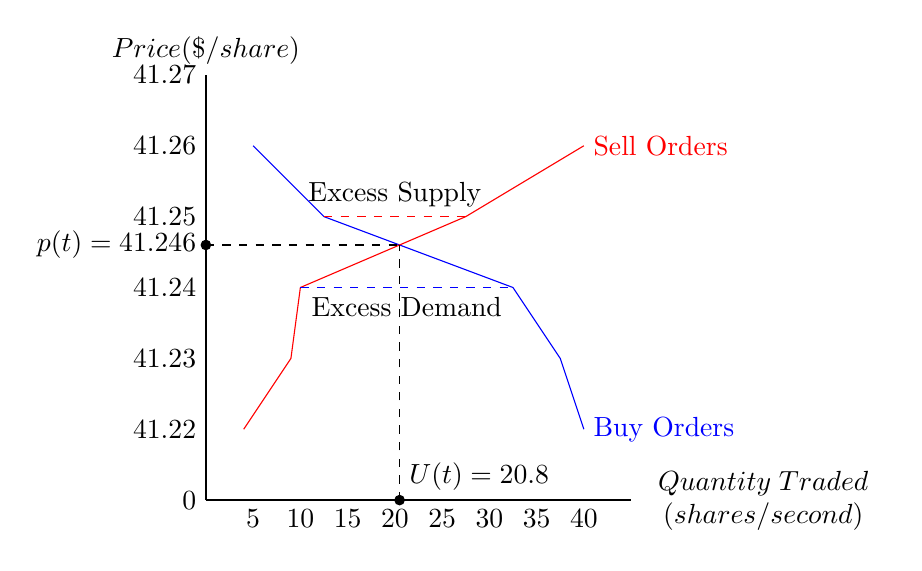
\begin{tikzpicture}[scale=0.6]
        \draw[thick,-] (0,0) -- (0,9) node[above]{$Price (\$/share)$};
        \draw[thick,-] (0,0)--(9,0) node[right]{\begin{tabular}{c}
             $Quantity \; Traded$ \\
             $(shares/second)$
        \end{tabular}};
        \node[left] at (0,1.5) {$41.22$};
        \node[left] at (0,3.0) {$41.23$};
        \node[left] at (0,4.5) {$41.24$};
        \node[left] at (0,6.0) {$41.25$};
        \node[left] at (0,7.5) {$41.26$};
        \node[left] at (0,9.0) {$41.27$};
        \node[below] at (1,0) {$5$};
        \node[below] at (2,0) {$10$};
        \node[below] at (3,0) {$15$};
        \node[below] at (4,0) {$20$};
        \node[below] at (5,0) {$25$};
        \node[below] at (6,0) {$30$};
        \node[below] at (7,0) {$35$};
        \node[below] at (8,0) {$40$};
        \node[left] at (0,0) {$0$};
        \draw[blue,solid] (1,7.5) -- (2.5,6.0) -- (6.5,4.5) -- (7.5,3) -- (8,1.5) node[right]{Buy Orders} ;
        \draw[red,solid] (0.8,1.5) -- (1.8,3) -- (2,4.5) -- (5.5,6) -- (8,7.5) node[right]{Sell Orders};
        \draw[red,dashed] (2.5,6.0) -- (5.5,6.0);
        \draw[blue,dashed] (2,4.5) -- (6.5,4.5);
        \node[black,above] at (4,6.0) {Excess Supply};
        \node[black,below] at (4.25,4.5) {Excess Demand};
        \draw[dashed] (4.1,0) -- (4.1,5.4);
        \draw[dashed] (0,5.4) -- (4.1,5.4);
        \node[above right] at (4.1,0) {$U(t)=20.8$};
        \draw[fill] (4.1,0) circle [radius=.1];
        \node[left] at (0,5.4) {$p(t)=41.246$};
        \draw[fill] (0,5.4) circle [radius=.1];
    \end{tikzpicture} \\
    \caption{\textbf{Flow supply, flow demand, and equilibrium in the Flow format.}
    \footnotesize In the example shown, excess supply = 28 - 12 = 16 shares at \$41.25 and excess demand = 34 - 10 = 24 shares at the next lower tick, \$41.24, so the clearing price is $\frac{41.24 ^* 16 \ + \ 41.25 ^* 24}{16 \ + \ 24}$ = \$41.246.
    }
    % \raggedright \footnotesize Note: Excess supply = 28 - 12 = 16 shares at \$41.25 and excess demand = 34 - 10 = 24 shares at the next lower tick, \$41.24, so the clearing price is $\frac{41.24 ^* 16 \ + \ 41.25 ^* 24}{16 \ + \ 24}$ = \$41.246.
    \label{fig:snd}
\end{figure}

The flow format enables traders to finely tailor their market engagement. Their chosen flow orders reflect not only their target prices but also their urgency of trading. It is not hard to see that the impact a flow order has on clearing price is reduced when a trader reduces her $U_{\max}$ or expands the width $p_H - p_L$ of her acceptable price range.  

\bigskip
\noindent
\textbf{Flow Trader Screen.} 
The software and interface for the Flow format parallels that for the CDA format. 
Figure \ref{fig:exp_interfaces}(b) shows an example of the user interface.  
The trader sets and submits buy and sell orders in the top-middle box (titled ``Your Input''). The horizontal axis denotes \textit{rate} in shares per second, and the vertical axis denotes prices in ECUs per share. 
The trader sets a \textit{buy} order by dragging the blue dot along the vertical axis to set the high price and dragging the blue square inside the grid to set the low price and the maximum rate. 
Then she enters the total number of shares she wants to buy in the box next to the ``Send Buy" blue button and submits it by clicking that button. The blue-line segments graphically describe her buy order. %, as shown in Figure \ref{fig:exp_interfaces} panel (b). 
Likewise, she sets a \textit{sell} order by moving the red dot along the vertical axis to set the low price and dragging the red square inside the grid to set the high price and the maximum rate. 
Then she enters the total number of shares she wants to sell in the box next to the ``Send Sell" red button and submits it by clicking that button. She can submit a new order at any time by canceling her active orders on the same side of the market and then creating a new order.\footnote{
Note that with our interface it takes only 
two drags, one click, and one textbox entry to submit a flow order. It is even simpler to submit a CDA order: one drag and one click suffice.}

The trader sees the market supply (the blue piecewise linear curve) and demand (red) in the top-right Market box. Their intersection determines the clearing price $p(t)$ and the aggregate clearing rate $q(t)$. The green horizontal line at height $p(t)$ in the Market diagram extends into the \textit{Your Input} box and indicates the current market price. The x-coordinate of the intersection of this line and the trader's order indicates the trader's current trading speed. The column of tables on the left side and the bottom boxes (projected profits, inventory, and cash) of the Flow interface parallel those in the CDA interface.  

\bigskip
\noindent
\textbf{Order constraints.} 
The market host (here, the experimenter) must specify the feasible price range and the maximum order size that can be processed.
For both formats we restrict submitted prices to be integers between 1 and 20, and require $Q_{max}$ to be an integer between 1 and 200. 
The Flow format also requires a minimum gap between $p_H$ and $p_L$, which we set to 1.0. 
Finally, the Flow format requires what we will call a speed limit, the maximum allowable $U_{max}$, which can be seen to be 30 shares per second in Panel (b) of Figure \ref{fig:exp_interfaces}. 
We selected that speed limit to make it unlikely that a single order would have a disproportionate impact.
Readers of an early draft suggested stress testing our markets with a higher speed limit, so the final Flow sessions double the speed limit to 60 shares per second.

% % \newpage
% \begin{figure}
%     \centering
%     \caption{Experiment Interfaces}
%     \begin{subfigure}[b]{\linewidth}
%         \centering
%         
\includegraphics[width=0.9\linewidth]{figures/cda_ui.png}
%         \caption{CDA Format}
%         \label{fig:cda_ui}
%     \end{subfigure}
%     \begin{subfigure}[b]{\linewidth}
%         \centering
%         
\includegraphics[width=0.9\linewidth]{figures/flow_ui.png}
%         \caption{FLOW Format}
%         \label{fig:flow_ui}
%     \end{subfigure}
%     \label{fig:exp_interfaces}
% \end{figure}
% % \newpage

\subsection{Design}\label{sect:design}

We use a between-group design with three arms: the Continuous Double Auction format (CDA), the Flow format with speed limit of 30 shares/sec (Flow30), and the Flow format with speed limit of 60 shares/sec (Flow60).
Each arm consists of five sessions, each with one market of eight traders, interacting in 20 trading periods of two minutes each. 
%That is, each CDA session has a identical twin Flow session with the same pattern of contract assignments, blocks, etc. as detailed below. 
At the start of each trading period,  four traders receive a single buy contract and four receive a single sell contract. %as each period starts. 
As mentioned above, %buy and sell contracts are analogous to induced values and costs in standard market experiments. In particular, 
a buy (sell) contract is a commitment from the experimenter to buy (sell) up to $Q_{C}$ units at price $p_{C}$ at the specified expiration time, here at the end of the trading period. % of the contract (all expiration times were set near the end of the trading period). \


We divide the 20 trading periods into five blocks of four consecutive periods each. 
The four periods within a block have the same contract configuration, i.e., the induced demand and supply curves repeat, and so do the equilibrium quantity and price. 
Such stationary repetition is traditional in market experiments and is intended to give traders the opportunity to discover equilibrium.

The contract configuration changes when the next block begins. 
The intention is to challenge the market to track a shifting equilibrium price and quantity.
We use the three different contract configurations depicted in Figure \ref{fig:3contract_configs_new}.
Configurations (a), (b) and (c) are used in Blocks one, two and three respectively.
Block four repeats the configuration of Block two, and Block five repeats that of Block one. 
The blue staircases in the Figure represent the buy contracts, sorted to form the induced demand curve, and the red supply curve similarly represents the sell contracts. 
Each contract assigned to an individual trader is a step (a flat line segment) on either demand or supply curve. 
In configuration (a), 
for example, one seller has $Q_{C}=400, p_{C}=3$ while another has $Q_{C}=400, p_{C}=4.$ 
The four buyers and the other two sellers all have 
$Q_{C}=300$ or 400; the other sellers' $p_C$'s are 11 and 14,
while the buyers' $p_C$'s are 17, 17, 16 and 14.
Contract information is private: each trader sees her own current contract but not those of other traders.

Within each block, each trader receives the same contract each period. Across blocks, buyers and sellers receive different contracts but keep the same role. The block structure is not announced; traders are simply told that their contracts may (or may not) change from one period to the next. 
% but we assign a new set of contacts as shown in Figure \ref{fig:3contract_configs_new}. 

%%%%% CONTRACT FIGURES %%%%%%%%%

\begin{figure}
    \centering
    % \caption{Contract Configurations}
    \begin{subfigure}[c]{0.33\linewidth}
        \centering
            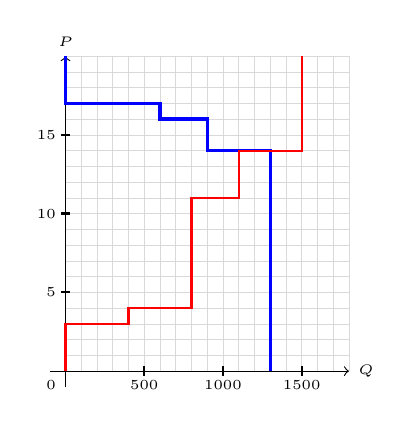
\begin{tikzpicture}[scale=.2]
                % create grid
                \draw[help lines, gray!30] (0,0) grid (18,20);
                
                % Draw axes
                \draw[->] (-1,0) -- (18,0) node[font=\tiny,right] {$Q$};
                \draw[->] (0,-1) -- (0,20) node[font=\tiny,above] {$P$};
              
                % Draw step functions
                \draw[blue, very thick] (0,20) -- (0,17) -- (6,17) -- (6,16) -- (9,16) -- (9,14) - - (13,14) -- (13,0) ;
                \draw[red, thick] (0,0) -- (0,3) -- (4,3) -- (4,4) -- (8,4) -- (8,11) --  (11,11) -- (11,14) -- (15,14) -- (15,20);
                
                % % Add labels
                \node[font=\tiny,below left] at (0,0) {$0$};
                \foreach \x in {5,10,15} {
                  \node[font=\tiny,below] at (\x,0) {$\x00$};
                }
                \foreach \y in {5,10,15} {
                  \node[font=\tiny,left] at (0,\y) {$\y$};
                }
                
                % % Add thicker ticks (Q)
                \draw[black, thick] (5,-0.3) -- (5,0.3);
                \draw[black, thick] (10,-0.3) -- (10,0.3);
                \draw[black, thick] (15,-0.3) -- (15,0.3);

                % % Add thicker ticks (P)
                \draw[black, thick] (-0.3,5) -- (0.3,5);
                \draw[black, thick] (-0.3,10) -- (0.3,10);
                \draw[black, thick] (-0.3,15) -- (0.3,15);
            \end{tikzpicture}
        \subcaption{\tiny Block 1 (T1-T4) \\ and Block 5 (T17-T20)}
    \end{subfigure}%
    \begin{subfigure}[c]{0.33\linewidth}
        \centering
        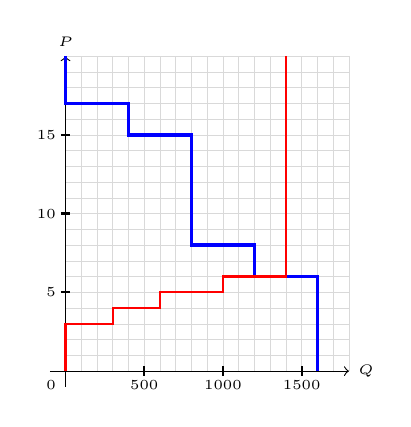
\begin{tikzpicture}[scale=.2]
            % create grid
            \draw[help lines, gray!30] (0,0) grid (18,20);
            
            % Draw axes
            \draw[->] (-1,0) -- (18,0) node[font=\tiny,right] {$Q$};
            \draw[->] (0,-1) -- (0,20) node[font=\tiny,above] {$P$};
          
            % Draw step functions
            \draw[blue, very thick] (0,20) -- (0,17) -- (4,17) -- (4,15) -- (8,15) -- (8,8) -- (12,8) -- (12,6) -- (16,6) -- (16,0);
            \draw[red, thick] (0,0) -- (0,3) -- (3,3) -- (3,4) -- (6,4) -- (6,5) -- (10,5) -- (10,6) -- (14,6) -- (14,20);
            
            % % Add labels
            \node[font=\tiny,below left] at (0,0) {$0$};
            \foreach \x in {5,10,15} {
              \node[font=\tiny,below] at (\x,0) {$\x00$};
            }
            \foreach \y in {5,10,15} {
              \node[font=\tiny,left] at (0,\y) {$\y$};
            }

            % % Add thicker ticks (Q)
            \draw[black, thick] (5,-0.3) -- (5,0.3);
            \draw[black, thick] (10,-0.3) -- (10,0.3);
            \draw[black, thick] (15,-0.3) -- (15,0.3);

            % % Add thicker ticks (P)
            \draw[black, thick] (-0.3,5) -- (0.3,5);
            \draw[black, thick] (-0.3,10) -- (0.3,10);
            \draw[black, thick] (-0.3,15) -- (0.3,15);
        \end{tikzpicture}
        \subcaption{\tiny Block 2 (T5-T8) \\ and Block 4 (T13-T16)}
    \end{subfigure}%
    \begin{subfigure}[c]{0.33\linewidth}
        \centering
        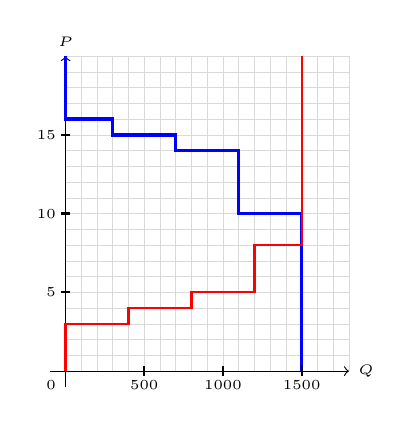
\begin{tikzpicture}[scale=.2]
            % create grid
            \draw[help lines, gray!30] (0,0) grid (18,20);
            
            % Draw axes
            \draw[->] (-1,0) -- (18,0) node[font=\tiny,right] {$Q$};
            \draw[->] (0,-1) -- (0,20) node[font=\tiny,above] {$P$};
          
            % Draw step functions
            \draw[blue, very thick] (0,20) -- (0,16) -- (3,16) -- (3,15) -- (7,15) -- (7,14) -- (11,14) -- (11,10) -- (15,10) -- (15,0);
            \draw[red, thick] (0,0) -- (0,3) -- (4,3) -- (4,4) -- (8,4) -- (8,5) -- (12,5) -- (12,8) -- (15,8) -- (15,20);
            
            % % Add labels
            \node[font=\tiny,below left] at (0,0) {$0$};
            \foreach \x in {5,10,15} {
              \node[font=\tiny,below] at (\x,0) {$\x00$};
            }
            \foreach \y in {5,10,15} {
              \node[font=\tiny,left] at (0,\y) {$\y$};
            }

            % % Add thicker ticks (Q)
            \draw[black, thick] (5,-0.3) -- (5,0.3);
            \draw[black, thick] (10,-0.3) -- (10,0.3);
            \draw[black, thick] (15,-0.3) -- (15,0.3);

            % % Add thicker ticks (P)
            \draw[black, thick] (-0.3,5) -- (0.3,5);
            \draw[black, thick] (-0.3,10) -- (0.3,10);
            \draw[black, thick] (-0.3,15) -- (0.3,15);
        \end{tikzpicture}
        \subcaption{\tiny Block 3 (T9 - T12)}
    \end{subfigure}
    \caption{\textbf{Contract configurations across trading blocks.}  \footnotesize
Vertical axis is price (ECU per share) and horizontal axis is quantity (shares). Each panel plots the step‐function demand schedule (thick blue) and supply schedule (red).  
The intersection of the two schedules determines the competitive‐equilibrium price–quantity pair for that block.  
Panel (a) applies to Blocks 1 (T1–T4) and 5 (T17–T20) of experiment; panel (b) to Blocks 2 (T5–T8) and 4 (T13–T16); panel (c) to Block 3 (T9–T12). }
% \label{fig:contract-configs}
    \label{fig:3contract_configs_new}
\end{figure}

% Yilin please add captions explaining the blocks and the equilibrium values. 

A few comments are in order about the chosen contract configurations. 
First, the rectangular shape of each contract matches the rectangular shape of an ordinary limit order, in that sense advantaging the CDA. % this facilitates comparable underlying incentives between the two market formats. 
Second, prior experimental evidence 
going back at least to \cite{friedman1995competitivity} suggests that efficiency in CDA markets tends to be lower (mainly due to undertrading) when goods are highly divisible; see \cite{angereretal}
for a recent confirmation.
% Investors’ Behaviors and Market Efficiency in Fractionalized Asset Markets by Martin Angerer, Marius Gramlich, and Yilong Xu, unpublished manuscript, University of Liechtenstein, Department Finance & Economics, August 2024
That tendency provides more room for either format to exhibit an efficiency advantage.
Third, the asymmetric surplus in panel (a) of Figure \ref{fig:3contract_configs_new} may lead to slow convergence to competitive equilibrium from below; indeed, excess demand for prices $p \in [11,14)$ below CE is only 1300 - 1100 = 200 shares, while excess supply at $p \in (14, 17]$ above CE is at least 1500 - 900 = 600 shares.
This asymmetry suggests that, in the first block, buyers will tend to make higher profits relative to CE than will sellers.
The second block provides a similar sort of advantage for seller profits, while the third block seems even-handed. As we will see below, those asymmetries indeed seem to influence market dynamics in the corresponding blocks. 
% but it may be that the initial pattern persists.


Experiment instructions are provided on the computer screen and in print; see online Appendix C for copies. %ces \ref{app_instruction_cda} and \ref{app_instruction_flow} for a copy. % Instructions were discussed and piloted (with students and colleagues) to balance clarity and reasonable length.} 
% \footnote{To ensure clarity and understanding of the experiment's rules and objectives, we provided participants with detailed instructions on-screen and paper, supplemented by a video summary. The experiment also included trial periods for participants to familiarize themselves with the interface and market rules. Final payments were based on accumulated wealth, incorporating a fixed participation fee.}
After 15 minutes of reading instructions, they are summarized in an animated and annotated video intended to aid participants' understanding. 
Two 120-second practice periods then familiarize participants with the interface and market rules; questions
are encouraged. 
The 20 actual trading periods then began.
Participants are not allowed to communicate with each other before or during the experiment, nor do they learn the identity or characteristics of other participants.

In between trading periods, each participant views a summary screen displaying the history of profits earned in previous trading periods.
% KLV Should we add a screen in the appendix?
Each participant starts each trading period with zero endowment. 
To simplify their task, they are not allowed to acquire inventory positions 
(short or long) beyond their contract quantity.
As explained in the instructions,
take-home pay consists of final cash
(after the experimenter fulfilled all contracts) each period summed across all twenty trading periods, and converted to US Dollars at a pre-announced exchange rate of 1000 ECUs = \$1, plus a \$7 participation fee. 
Negative earnings are quite rare, occurring in less than 5\% of periods and never for an entire session. 
%4.62\% of the cases (4.88\% in the CDA and 4.37\% in FLOW)
Payments are made privately and average \$28.77 per participant %, with a %minimum of \$13.68 and maximum of \$51.99. (std = 
(standard deviation \$8.38).
The experiment software is built on the oTree platform \citep{otree}. Sessions are conducted at the LEEPS Laboratory of the University of California, Santa Cruz and last 100 minutes on average. Participants are recruited via LEEPS' ORSEE instance (\hyperlink{https://econlab.ucsc.edu/public/}{econlab.ucsc.edu}; \cite{Greiner2015}).


% \subsection{Hypotheses}
% list the criteria we will use for market quality  --- 
% allocative efficiency, price efficiency, price volatility, profit level and dispersion, ... ---
% and for each criterion offer a hypothesis on which format will be better.

% describe in words how we defined?
%%%%%%%%%%%%%%%%%%%%%%%%%%%%%%%%%%%%%%%%%%%%%%%%%%%%%%%%%%%%%%%%%%%%%%%%%%%%%%%%%%%%%%%%%%%%%%%%%%%%%%%%%%%%%%%%%%%
\subsection{Performance Metrics and Hypotheses}\label{sect:metricHyps}
\label{sec:hypotheses}

To compare the two market formats, we will analyze \textbf{trader behavior} in terms of 
the \textit{number of submitted orders} per trading period, 
the \textit{size of submitted orders}  in shares per order,
the \textit{prices} of submitted orders, and, for Flow trading, 
the \textit{maximum trading rate}.

We will also analyze \textbf{market performance} using several metrics.
\textit{Absolute Price Change} is defined for each period as the average absolute difference in transaction prices between adjacent time grid points, $|P_t - P_{t-1}|$. A larger value indicates more erratic prices. 
Our convention on
the (5-second) time grid is described below. %lower price volatility. %\footnote{We define trading intervals at the beginning of the Results section.}
\textit{Price volatility} is defined for each period as the variability of proportional price changes across time grid intervals, and is calculated as the standard deviation of $(\ln P_t - \ln P_{t-1})$.
%periods and groups. This is another metric of price volatility. 
A new liquidity metric called 
\textit{Price pressure index (PPI)} is defined each period as the average across time intervals of the per-share cost of executing a buy-sell round trip of a standard package ($Q^* = 20$ shares). %in a short time interval ($\Delta t = 5$ seconds). 
A lower PPI indicates less impact on price and thus greater liquidity; see Appendix A for technical details.  

Other market performance metrics are computed once per period.
\textit{Trade Volume} is defined  as the total quantity of shares traded in a period. An aggregate indicator of market activity, it can be compared to the minimum trading volume required to achieve a competitive equilibrium allocation. An alternative volume metric is \textit{Filled Contract}, the quantity filled by the experimenter when contracts expire; this metric ignores volume due to ``churn,'' e.g.,  traders reselling part of their purchases.
\textit{Informational [in]efficiency} is  defined each period as the mean absolute deviation of transaction price from the  competitive equilibrium price, \( |P_t - P_{\text{CE}}| \). 
Smaller deviations indicate higher informational efficiency, that is, transaction prices that more fully incorporate all private information regarding supply and demand.\footnote{
Thus, in the CE benchmark, \( |P_t - P_{\text{CE}}| \), $|P_t - P_{t-1}|$ and 
$(\ln P_t - \ln P_{t-1})$ are all zero.}
Finally, \textit{Allocative efficiency} is measured as \( \Pi/\Pi_{\text{CE}}\), i.e.,
 realized surplus (the sum of traders' actual profits) as a fraction of potential surplus (the sum of trader profits earned in competitive equilibrium). 
This metric assesses how efficient the market is in extracting potential gains from trade.       


%%%%%%%%%%%%%%%%%%%%%%%%%%%%%%%%%%%%%%
% \vspace{0.5cm}
% \noindent \textit{Hypotheses} \\

Those metrics allow us to formulate the following testable hypotheses. 

%\vspace{0.3cm}
\noindent \textbf{Hypothesis 1: Order shredding.} \textit{Traders will submit a larger number of smaller quantity orders in the CDA format than in the Flow format.} 
%\vspace{0.3cm}

\noindent As discussed earlier, to reduce price impact in the CDA, traders have to shred their orders manually, i.e., to break the overall quantity to be traded into fragments submitted sequentially. By contrast, the Flow format automatically facilitates very fine order shredding since, in each short time interval, only a very limited quantity can be transacted. 
The Flow format can closely reproduce CDA trading and pricing dynamics if traders set $U_{\text{max}}$ at the speed limit (30 or 60) while setting $p_H= p_L+1,$ minimizing the price separation. 
If traders instead modulate their urgency to trade --- by choosing a wide gap between prices $p_L$ and $p_H$  and/or choosing $U_{\text{max}}$ well below the speed limit --- then they automatically will greatly reduce price impact even when they submit large orders. Thus, if traders care about price impact,\footnote{\cite{elenaetal} find that, with highly divisible assets, traders in a CDA may shred orders for reasons beyond price impact. 
Specifically, traders may wish to hedge their bets early in the trading period against the possibility of more favorable prices later in the period. Such a diversification motive would not seem very sensitive to the market format, but it suggests that orders may be earlier, fewer and larger in later periods when traders have less uncertainty about price distributions.} 
in the Flow format we should observe fewer but larger orders than in the CDA. 

\vspace{0.3cm}
\noindent \textbf{Hypothesis 2: Volatility.} \textit{Price volatility will be lower with the Flow format than with the CDA format.}
%\vspace{0.3cm}

\noindent In the CDA, each transaction is executed at a price determined by a unique bilateral matching of limit orders of a buyer and a seller. This can lead to a wide dispersion of transaction prices within a short time interval. In contrast, the Flow Market operates under a uniform pricing rule — from moment to moment, every trade for every active trader is executed at the same price, until an active order is fully filled or a new order arrives. This uniformity may attenuate transaction price fluctuations, yielding a more stable price path. Hence, we hypothesize that the Flow format brings lower price volatility than the CDA. 


\vspace{0.3cm}
\noindent \textbf{Hypothesis 3: Liquidity.} \textit{ PPI will be lower, i.e., markets will be more liquid, with the Flow format than with the CDA format.}

\noindent 
If the Flow format indeed reduces price volatility and the need to manually shred orders, then it should encourage traders to place larger bids and asks in the order book closer to the current clearing price. Such enhanced liquidity would reduce the round-trip cost of a modest order to buy and resell, i.e., it would reduce PPI. 
%The Flow Market is designed to automatically shred orders and execute trades at a more consistent rate relative to the CDA, and at a less volatile uniform price (see previous hypothesis). This should reduce the immediate impact of large orders on prices, leading to lower price pressure. It is then expected that the Flow Market will exhibit a lower Price Pressure Index (PPI). 

\vspace{0.3cm}
\noindent \textbf{Hypothesis 4: Volume.} \textit{The CDA and Flow formats will exhibit similar levels of trade volume. }
%(b) Both will move within each trading block towards the minimum volume that sustains competitive equilibrium.} 
%\vspace{0.3cm}

\noindent There is no obvious reason in our environment\footnote{
{By contrast}, in the environment currently experienced in major financial markets, it is typically the case that natural buyers transact with HFT traders, who transact with natural sellers. Thus trading volume is about double what it would be in markets 
(perhaps including Flow) in which natural buyers transact directly with natural sellers.
CDA volume is also boosted by HFT races for latency arbitrage \citep{AquilinaBudishOneill2022}.}
why the overall trade volume should be larger in one format than the other, so H4 is the natural null hypothesis. We shall also examine whether trade volume in later periods approaches the competitive equilibrium volume. 

\vspace{0.3cm}
\noindent \textbf{Hypothesis 5: Efficiency.} \textit{The CDA and Flow formats will exhibit similar levels of (a) informational and (b) allocative efficiency.} 
%\vspace{0.3cm}

\noindent Again, there is no compelling reason in our simple environment\footnote{
Note this is not necessarily true in environments such as \cite{Budish2015} and \cite{Aldrich2019} where equilibrium in the CDA implies socially wasteful investment in technology.}
to expect one format to be more efficient than the other, either in informational efficiency (prices close to competitive equilibrium) or in allocative efficiency (exhaustion of gains from trade), 
so H5 is the natural null hypothesis. 

% On the other hand, proponents of either format would be happy to see this hypothesis rejected in their preferred direction.

%%%%%%%%%%%%%%%%%%%%%%%%%%%%%%%%%%%%%%%%%%%%%%%%%%%%%%%%%%%%
%%%%%%%%%%%%%%%%%%%%%%%%%%%%%%%%%%%%%%%%%%%%%%%%%%%%%%%%%%%%


\begin{table}[t]
%\begin{table}[!htbp]
    \centering
    \caption{Summary Statistics: Traders' Behavior.}
    \label{tab:summary_stat_trader}
    %\renewcommand{\arraystretch}{1}
    \resizebox{.8\textwidth}{!}{
    \begin{threeparttable}
    \begin{tabular}{lcccccc}
    \toprule
    ~                               & \multicolumn{3}{c}{---------All Periods---------} & \multicolumn{3}{c}{---------Second Half-----------} \\
                                    & CDA       & Flow30      & Flow60      & CDA       & Flow30     & Flow60     \\
    \midrule 
     Number of Orders               & 32       & 24            & 26            & 32        & 23            & 25            \\
    \hspace{3mm}Seller              & 17       & 12            & 13            & 17        & 11            & 12            \\
    \hspace{3mm}Buyer               & 15       & 12            & 13            & 15        & 12            & 12            \\
 \hline
     Shares per Order               & 114      & 186           & 192           & 112       & 188           & 195           \\
    \hspace{3mm}Seller              & 115      & 185           & 191           & 111       & 185           & 197           \\
    \hspace{3mm}Buyer               & 114      & 188           & 193           & 113       & 191           & 193           \\
   \hline
     Order Price                    & 8.8      & [6.7, 12.6] & [6.9, 11.8] & 8.5      & [6.4, 12.3]  & [7.0, 11.7] \\
    \hspace{3mm}Seller              & 10.7     & [9.2, 15.5] & [9.4, 14.1] & 10.3     & [8.7, 14.9] & [9.3, 13.6] \\
    \hspace{3mm}Buyer               & 6.9      & [4.2, 9.7]  & [4.4, 9.5]  & 6.8      & [4.2, 9.7]  & [4.6, 9.8]  \\
   \hline
     Order Max Rate                 &          & 19.91         & 34.11         &           & 21.83         & 36.83         \\
    \hspace{3mm}Seller              &          & 19.67         & 35.82         &           & 21.29         & 39.3          \\
    \hspace{3mm}Buyer               &          & 20.15         & 32.4          &           & 22.37         & 34.36         \\
   \hline
    Orders at Max Quantity          & 0.26     &               &               & 0.26      &               &               \\
    \hspace{3mm}Seller              & 0.25     &               &               & 0.25      &               &               \\
    \hspace{3mm}Buyer               & 0.27     &               &               & 0.26      &               &               \\
   \hline
    Orders at Speed Limit      &          & 0.38          & 0.22          &           & 0.48          & 0.29          \\
    \hspace{3mm}Seller              &          & 0.38          & 0.23          &           & 0.46          & 0.30           \\
    \hspace{3mm}Buyer               &          & 0.39          & 0.21          &           & 0.49          & 0.27          \\
    \bottomrule
    \end{tabular}
%     \begin{tablenotes}
% \item \footnotesize \textit{Notes:} 
% \caption{Summary Statistics: Traders' Behavior. 
% {\footnotesize
% }}
\begin{tablenotes}[para,flushleft]
\footnotesize
\textit{Note:} 
All Periods columns (or Seond Half columns) report averages over all 20 periods (or last 10 periods) of each session. 
CDA columns (or Flow30 or Flow60 columns) report averages over sessions using the Continuous Double Auction (or Flow with speed limit = 30 or 60) format. 
Shares per Order is the number of shares $Q$ in a submitted order. 
Order Price is the limit price in submitted CDA orders, and bracketed prices are low and high prices $[p_L, p_H ]$ in submitted Flow orders. 
Order Max Rate refers to the maximum trading speed $U_{max}$ specified in a Flow order. 
Orders at Max Quantity gives the fraction of submitted orders with $Q_{max} = 200$. 
Orders at Speed Limit gives the fraction of submitted Flow Market orders whose $U_{max}$ is at the speed limit.
\end{tablenotes}
%\end{tablenotes}
\end{threeparttable}
}
\end{table}

\vspace{-.15in}
\section{Results} \label{results}
\vspace{-.15in}
We start with broad descriptive statistics of trader behavior and market performance. Section II.\ref{sect:FlowCDFnScatters} probes behavior in the Flow market a bit more deeply.
Section II.\ref{sect:RegResults} presents regression results, including formal tests of Hypotheses H1 - H5.

\subsection{Descriptive Analysis}

\noindent \textbf{Trader Behavior.} 
Table \ref{tab:summary_stat_trader} suggests that trader behavior in the Continuous Double Auction (CDA) 
diverges from that in the Flow Market format. 
CDA markets have an overall average of 32 orders per period, while the Flow markets average only 24 or 26 orders. 
On the other hand, the Flow orders are substantially larger on average, at 186 or 192 shares 
(rather close to the 200 share limit), versus 114 shares in CDA markets. This divergence persists in  late (T11-20) periods and for Buyers as well as Sellers. Although not a formal test of H1, the descriptive statistics suggest that indeed the Flow market's automatic shredding helps traders reduce price impact without having to chop up their orders manually.  

The rest of the Table shows both similarities and differences in pricing behavior. 
Bid prices in CDA limit orders average 6.9 ECU per share, while Flow bid prices with the regular speed limit (Flow30) stretch from an average low price of 4.2 to an average high price of 9.7,
and similarly from 4.4 to 9.5 in Flow60.  
Thus the CDA average submitted bid is right in the middle of average bid intervals in Flow markets. However, for sellers' asks, the CDA limit prices are, on average, much closer to the lower end of Flow market price interval.  
We will see later that this order price asymmetry connects with profit asymmetries between buyers and sellers. 


% \begin{figure}[!h] 
%     \centering
%     \begin{subfigure}[b]{\linewidth}
%         \centering
%         % \begin{adjustbox}{trim=0 {.02\height} 0 {.12\height}, clip=true}
%         \begin{adjustbox}{trim=0 {.02\height} {.10\width} {.11\height},clip=true}
%             
\includegraphics[width=1\linewidth]{new plots/groups_cda_price.png}
%         \end{adjustbox}
%         \subcaption{CDA}
%     \end{subfigure}
%     \begin{subfigure}[b]{\linewidth}
%         \centering
%         \begin{adjustbox}{trim=0 {.02\height} {.10\width} {.11\height},clip=true}
%             
\includegraphics[width=1\linewidth]{new plots/groups_flow_price_r.png}
%         \end{adjustbox}
%         \subcaption{Flow30}
%     \end{subfigure} 
%     \begin{subfigure}[b]{\linewidth}
%         \centering
%         \begin{adjustbox}{trim=0 {.02\height} {.10\width} {.11\height},clip=true}
%             
\includegraphics[width=1\linewidth]{new plots/groups_flow_price_s.png}
%         \end{adjustbox}
%         \subcaption{Flow60}
%     \end{subfigure} 
% \caption{\textbf{Transaction prices over time.} \footnotesize Faint colored lines (for Flow markets in Panels (b-c)) or dots (for CDA markets in Panel (a)) indicate prices in each individual session, and dark green lines or dots are averages across the 5 sessions in each format. The purple line represents the underlying competitive equilibrium price for each block of periods. Vertical dotted lines separate the 20 paid periods.
% % \textcolor{red}{the block and period numbers are too faint to see easily..} 
% }    
%     \label{fig:price}
% \end{figure}


%%%%%%%%%%%%% YL: updated below
\begin{figure}[!h] 
    \centering
    \begin{subfigure}[b]{\linewidth}
        \centering
        % \begin{adjustbox}{trim=0 {.02\height} 0 {.12\height}, clip=true}
        \begin{adjustbox}{trim=0 {.02\height} {.10\width} {.11\height},clip=true}
            
\includegraphics[width=1\linewidth]{plots (Nov 25)/groups_cda_price_single.png}
        \end{adjustbox}
        \subcaption{CDA}
    \end{subfigure}
    \begin{subfigure}[b]{\linewidth}
        \centering
        \begin{adjustbox}{trim=0 {.02\height} {.10\width} {.11\height},clip=true}
            
\includegraphics[width=1\linewidth]{plots (Nov 25)/groups_flow30_price_single.png}
        \end{adjustbox}
        \subcaption{Flow30}
    \end{subfigure} 
    \begin{subfigure}[b]{\linewidth}
        \centering
        \begin{adjustbox}{trim=0 {.02\height} {.10\width} {.11\height},clip=true}
            
\includegraphics[width=1\linewidth]{plots (Nov 25)/groups_flow60_price_single.png}
        \end{adjustbox}
        \subcaption{Flow60}
    \end{subfigure} 
    \caption{\textbf{Transaction prices over time.} \footnotesize Dark green lines (for Flow markets in Panels (b-c)) or dots (for CDA markets in Panel (a)) indicate average prices across the 5 sessions in each format. The purple line represents the underlying competitive equilibrium price for each block of periods. Vertical dotted lines separate the 20 paid periods.
    % \textcolor{red}{the block and period numbers are too faint to see easily..} 
    }    
    \label{fig:price}
\end{figure}



It is also worth noting that the wide difference between average minimum and maximum order prices, for both buyers and sellers, suggests that traders indeed seize the richer possibilities the Flow format provides to express immediacy (or patience). 
That impression is reinforced by the fact that the average maximum rates in the Flow buy and sell orders are well short of the speed limit. 
For example, in the Second Half (periods 11-20), the average $U_{max}$ in submitted orders is about 37 shares per second in Flow60 where the speed limit is 60. 
That said, there is a tendency towards higher $U_{max}$ in later periods;
e.g., in Flow30 (resp. Flow60) 48\% of submitted orders are at the speed limit in Second Half vs 38\% overall (resp. 29\% in Second Half vs 22\% overall).
Thus in the Flow format, traders seemingly become a bit more aggressive over time in the speed dimension. Buyers show little trend in the price dimension.
Sellers price slightly more aggressively in Second Half than overall,
reducing the asymmetry noted in the previous paragraph.
There is no obvious trend in CDA traders' expressed urgency: both buyers and sellers, in later periods and overall, place about about a quarter of their orders for 200 shares, the maximum allowed.

% Market Performance
\vspace{0.5cm}
\noindent \textbf{Market Performance.} 
Figure \ref{fig:price} displays session-average prices over time, within and across periods. Panel (a)
shows rather wide price fluctuations within the CDA (dark green dots), but on average  prices tend to under-react to changes in the competitive equilibrium (CE) price. 
In a few periods (e.g., periods 8 and 14-16) prices almost converge to CE, but for the most part they tend to fall below CE in blocks 1, 3 and 5, and to remain above CE in block 2. 
With the exception of block 3, that tendency was anticipated in the contract configuration discussion in Section I.\ref{sect:design}.
Panels (b) and (c) show roughly similar tendencies in the Flow markets. 
Average prices across sessions (dark green lines) seem perhaps a bit less erratic than in the CDA.
Flow market prices are closer to the CE benchmark in block 3 
and perhaps have a greater tendency to approach the CE level towards the end of the period in blocks 1, 2 and 5. 
Overall, in our challenging environment, 
prices in all formats seem weakly responsive to the block-by-block changes in CE price. 




\begin{table}[!h]
%\begin{table}[t]
    \centering
    \caption{Summary Statistics: Market Performance.}
    \label{tab:summary_stat}
    \renewcommand{\arraystretch}{0.9}
     \resizebox{.95\textwidth}{!}{
    \begin{threeparttable}
    \begin{tabular}{lcccccc}
    
    \toprule
    
    ~           & \multicolumn{3}{c}{------All Periods------} & \multicolumn{3}{c}{------Second Half------} \\
                & CDA       & Flow30    & Flow60     & CDA      & Flow30    & Flow60 \\
    \midrule 
     \\[-1.8ex] 
     \multicolumn{7}{l}{\textit{\textbf{Panel A.} Price Statistics} (Avg. Equil Price = $9.80$ ECUs)} \\
    % \hline  
     \\[-1.8ex]    
     Clearing Price ($P_\tau$)           & 8.62     & 9.37     & 9.45    & 8.21      & 9.18      & 9.29      \\
    \hspace{3mm}(Std. Dev.)                     & (2.77)   & (2.54)   & (2.14)   & (2.51)    & (2.29)    & (2.01)    \\
     $ \lvert  P_{\tau} - P_{\tau - 1} \rvert $ & 0.57     & 0.39     & 0.43     & 0.55      & 0.4       & 0.43      \\
     Volatility & 0.14     & 0.07     & 0.08     & 0.13      & 0.07      & 0.08      \\
     Price Pressure Index (PPI)      & 3.98      & 0.89        & 0.78       & 3.88      & 0.76     & 0.68      \\
     \\ [-1.8ex]
     \multicolumn{7}{l}{\textit{\textbf{Panel B.} Volume, Transaction Intensity}} \\
     \\ [-1.8ex]
   
     Trade Volume (shares)                     & 1138      & 959       & 1121    & 1179      & 1046      & 1175     \\
     Trade Vol. / $Q_{\text{CE}}$ (\%)        & 93.6      & 78.8      & 92.1    & 96.9      & 86.4     & 96.8   \\
     Filled Contract / $Q_{\text{CE}}$ (\%)     & 85.2      & 77.1    & 88.1      & 89.3      & 84.5   & 91.8   \\
     Num. of Transactions                             & 14        &        &   & 15        &      &     \\
     Mean Transaction Size                      & 78        &         &  & 74        &        &   \\
     \hspace{3mm}(Std. Dev.)             & (61)      &      &     & (60)      &       &    \\
     Clearing Rate ($q/sec$)                 &           & 9.37      & 9.69     &           & 9.20       & 9.51     \\
     
     \hspace{3mm}(Std. Dev.)             &           & (2.6)    & (2.42)     &           & (2.4)     & (2.13)   \\
      Time with no Flow (\%)               &           & 11      & 12    &           & 10        & 11   \\

     \\ [-1.8ex]
     \multicolumn{7}{l}{\textit{\textbf{Panel C.} Efficiency and Buyer-Seller Inequality}} \\
     \\ [-1.8ex]
     
     Info. Effic.: $\lvert P_t - P_{\text{CE}} \rvert $        & 2.16      & 2.08    & 2.18  & 2.14      & 1.84    & 2.14  \\     
     Alloc. Effic.: $\Pi$ / $\Pi_{\text{CE}}$ (\%)   & 84.3      & 81.81    & 90.04     & 88.85     & 86.31     & 93.55   \\
     
     ${\Pi^{\text{buy}}}/{\Pi^{\text{buy}}_{\text{CE}}} - {\Pi^{\text{sell}}}/{\Pi^{\text{sell}}_{\text{CE}}}$ 
     (\%) & 53.7      & 11.18    & 9.97    & 80.03     & 27.51    & 17.17    \\
     \\[-1.8ex] 
    \bottomrule
    \end{tabular}
    \begin{tablenotes}[para,flushleft]
\footnotesize
\textit{Note:} 
All Periods includes T1-20 and Second Half includes T11-20.
Prices are quantity-weighted within 5-second time intervals.
Table entries are averages over all relevant periods and sessions. 
$|P_{\tau} - P_{\tau-1}|$ is average absolute price change between successive time intervals. 
Volatility is the standard deviation of $\left( \ln P_{\tau} - \ln P_{\tau-1} \right)$, the proportional price change between time intervals. 
PPI is the per-share round-trip cost of a standard package ($Q^* = 20$ shares) in the time interval.
Trade Vol / $Q_{CE}$ (\%) is the average total quantity transacted per period as a percentage of the minimum required to reach competitive equilibrium (CE). 
Filled Contract / $Q_{CE}$ (\%) is the total quantity redeemed when contracts expire as a percentage of CE quantity.
Number of Transactions and Mean Transaction Size are CDA averages rounded to nearest integer. 
Clearing Rate is average market-level transaction rate in Flow trading. 
    Time with No Flow (\%) is percentage of time intervals with zero clearing rate. 
    Informational inefficiency, $|P_{\tau} - P_{CE}|$, and allocation efficiency, $ \Pi/\Pi_{CE} \times 100$ are averaged across trading periods.
    The last line is profit asymmetry, the difference $(\Pi^{buy}/\Pi^{buy}_{CE} - \Pi^{sell}/\Pi^{sell}_{CE})$ in normalized profits between buyers and sellers, expressed as a percentage. 
    \end{tablenotes} 
\end{threeparttable}

   }
\end{table}

Table \ref{tab:summary_stat} presents summary statistics of market performance. To facilitate comparisons between the different formats, we split each trading period into twenty-four consecutive 5-second intervals,\footnote{We also reconducted the analysis with 2-second and 10-second intervals. Online Appendix B.1-B.2 shows that the results are qualitatively similar.}
and within each interval we compute quantity-weighted average transaction prices.  %displayed in Figure \ref{fig:price}.
Panel A of Table \ref{tab:summary_stat} %details the average prices and their volatility. The Flow market exhibits 
shows higher average transaction prices in Flow markets, at 9.37 and 9.45 ECUs, compared to the CDA average of 8.62; they all fall a bit below the average competitive equilibrium (CE) price of 9.8. 

The Table strongly suggests greater price stability with the Flow format. 
Overall average absolute price change (\(|P_\tau - P_{\tau-1}|\)) across time intervals is 0.39 and 0.43 ECUs for Flow30 and Flow60 versus 0.57 for CDA. 
The contrast in average price volatility (standard deviation of log price changes) is even sharper:
just 0.07 and 0.08 in Flow30 and Flow60 versus 0.14 in CDA.
Both contrasts remain in later trading periods. %These figures show consistently lower volatility in price changes in the Flow market, pointing at traders in Flow experiencing a more predictable price evolution. 
Even more striking, the price pressure index (PPI) is much lower in Flow markets than in CDA, suggesting much better liquidity and lower trading costs. 


% \begin{figure}[!h]
%     \centering
%     \captionsetup[subfigure]{justification=centering}
%     %======================  Row 1 :  CDA  ======================%
%     \begin{subfigure}[b]{.48\linewidth}
%         \centering
%         \begin{adjustbox}{trim=0 {.02\height} {.05\width} {.11\height},clip,max width=\linewidth}
%             
\includegraphics{figures/groups_cda_quantity.png}
%         \end{adjustbox}
%         \subcaption{CDA — Traded Volume}
%         \label{fig:cda_volume}
%     \end{subfigure}
%     \hfill
%     \begin{subfigure}[b]{.48\linewidth}
%         \centering
%         \begin{adjustbox}{trim=0 {.02\height} {.05\width} {.11\height},clip,max width=\linewidth}
%             
\includegraphics{figures/groups_cda_surplus.png}
%         \end{adjustbox}
%         \subcaption{CDA — Surplus}
%         \label{fig:cda_surplus}
%     \end{subfigure}
%     \par\medskip
%     %======================  Row 2 :  Flow30  =====================%
%     \begin{subfigure}[b]{.48\linewidth}
%         \centering
%         \begin{adjustbox}{trim=0 {.02\height} {.05\width} {.11\height},clip,max width=\linewidth}
%             
\includegraphics{new plots/groups_flow_quantity_r.png}
%         \end{adjustbox}
%         \subcaption{Flow30 — Traded Volume}
%         \label{fig:flowr_volume}
%     \end{subfigure}
%     \hfill
%     \begin{subfigure}[b]{.48\linewidth}
%         \centering
%         \begin{adjustbox}{trim=0 {.02\height} {.05\width} {.11\height},clip,max width=\linewidth}
%             
\includegraphics{new plots/groups_flow_surplus_r.png}
%         \end{adjustbox}
%         \subcaption{Flow30 — Surplus}
%         \label{fig:flowr_surplus}
%     \end{subfigure}
%     \par\medskip
%     %======================  Row 3 :  Flow60  =====================%
%     \begin{subfigure}[b]{.48\linewidth}
%         \centering
%         \begin{adjustbox}{trim=0 {.02\height} {.05\width} {.11\height},clip,max width=\linewidth}
%             
\includegraphics{new plots/groups_flow_quantity_s.png}
%         \end{adjustbox}
%         \subcaption{Flow60 — Traded Volume}
%         \label{fig:flows_volume}
%     \end{subfigure}
%     \hfill
%     \begin{subfigure}[b]{.48\linewidth}
%         \centering
%         \begin{adjustbox}{trim=0 {.02\height} {.05\width} {.11\height},clip,max width=\linewidth}
%             
\includegraphics{new plots/groups_flow_surplus_s.png}
%         \end{adjustbox}
%         \subcaption{Flow60 — Surplus}
%         \label{fig:flows_surplus}
%     \end{subfigure}
%     %--------------------  Caption  ------------------------------%
%     \caption{\textbf{Trade volume and realized surplus.} \footnotesize   Faint colored lines show observed volume (in shares) and realized surplus (as \% of the CE surplus) for each of the 20 periods of each session; dark green lines show averages across sessions; and the pink step function shows the competitive‐equilibrium (CE) volume (or normalized surplus, for the horizontal pink line) in each block. Analogous plots for filled contracts appear in  Appendix Figure~\ref{fig:contract-fill}. 
%     }
%     \label{fig:volume_surplus_grid}
% \end{figure}


%%%%%%%%%% YL: updated below
\begin{figure}
    \centering
    \begin{subfigure}[b]{.5\linewidth}
        \centering
        \begin{adjustbox}{trim=0 0 0 {0.0\height}, clip=true}
            
\includegraphics[width=\linewidth]{plots (Nov 25)/groups_mean_quantity.png}
        \end{adjustbox}
       % \subcaption{\tiny Traded Volume}
    \end{subfigure}%
    \begin{subfigure}[b]{.5\linewidth}
        \centering
        \begin{adjustbox}{trim=0 0 0 {0.0\height}, clip=true}
            
\includegraphics[width=\linewidth]{plots (Nov 25)/groups_mean_surplus.png}
        \end{adjustbox}
        %\subcaption{\tiny Surplus}
    \end{subfigure}
    \caption{\textbf{Trade volume and realized surplus.} \footnotesize Panel (a) shows the observed volume (in shares) for each of the 20 periods averaged across sessions. Panel (b) shows similar averages for realized surplus as a fraction of competitive equilibrium (CE) surplus. 
    The pink step function (or horizontal dashed line in Panel (b)) shows the minimal CE volume (or the normalized CE surplus) in each block.}
    \label{fig:volume_surplus}
\end{figure}

The volume and transaction intensity measures shown in Panel B of Table \ref{tab:summary_stat} may also be of interest.
Gross volume is similar in CDA and Flow60, but lower in Flow30
especially in early rounds.
On the other hand, when we eliminate churn in the Filled Contract metric, volume is highest in Flow60, reaching almost 92\% of the CE level in the later trading periods.  
This suggests a steeper learning curve for traders in the Flow format. 
It also suggests that volume in both formats is converging towards CE levels, perhaps more so for CDA and Flow60 than Flow30; 
Figure \ref{fig:volume_surplus}a
confirms that impression.


The number of CDA transactions per period increases only slightly from 13 in the first ten periods of a session to 15 in the last ten. On the other hand, mean CDA transaction size decreases more substantially to 74 shares in the last ten periods (albeit with considerable variability; the coefficient of variation ($\frac{Std. Dev}{Mean}$) is around 0.75.) 
This suggests that order shredding may increase modestly
over time in the CDA.
In Flow markets the average clearing rate remains far below the upper speed limit of 30 or 60 shares per second, decreasing modestly to 9.20 or 9.51 in the second half of a session. 
The percentage of idle time in Flow markets %(time intervals with zero trading rate) 
is low, only about 10\% in later periods. 

Panel C of Table \ref{tab:summary_stat} reports efficiency metrics. Recall that informational (in)efficiency, $\lvert P_t - P_{\text{CE}} \rvert $, captures the market's capacity to track equilibrium price, while allocative efficiency,  $\Pi$ / $\Pi_{\text{CE}}$ (\%), is the percentage of potential surplus that is realized in each trading period. The Table indicates that Flow30 has better informational efficiency, with price deviating only by 1.84 on average in later periods,
while average deviations in CDA and Flow60 stagnate at 2.14.
On the other hand, the Table suggests that Flow60 has the best allocative efficiency in our challenging environment, enabling traders to reap over 93\% of mutual gains in later periods, while average efficiency 
in CDA and in Flow30 remains below 90\%. 

Finally, Panel C of Table \ref{tab:summary_stat} and Figure \ref{fig:norm_profits} show buyer vs seller  profits across market formats. Buyers' normalized profits greatly exceed sellers' profits in the CDA, but the profit asymmetry is much smaller in the Flow formats. 
Figure~\ref{fig:norm_profits} shows more detail. 
For example, about 70\% of CDA sellers earn less than their CE profit, while many buyers earn considerably more:
almost 20\% of CDA buyers earn at least two and a half times the CE profits.
The distributions of Flow profits are all less extreme.

% \begin{figure}
%     \centering
%     \begin{subfigure}[b]{.5\linewidth}
%         \centering
%         \begin{adjustbox}{trim=0 0 0 {0.0\height}, clip=true}
%             
\includegraphics[width=\linewidth]{new plots/group_gross_profits_cdf.png}
%         \end{adjustbox}
%         \subcaption{\tiny T1-T20}
%     \end{subfigure}%
%     \begin{subfigure}[b]{.5\linewidth}
%         \centering
%         \begin{adjustbox}{trim=0 0 0 {0.0\height}, clip=true}
%             
\includegraphics[width=\linewidth]{new plots/group_gross_profits_last_cdf.png}
%         \end{adjustbox}
%         \subcaption{\tiny T11-T20}
%     \end{subfigure}
%     \caption{\textbf{Profit distribution.} \footnotesize Panel (a) shows the period-level distribution of profits for the first half of the session and Panel (b) for the second half. We separate the empirical cumulative distributions by market role (seller and buyer) market format (CDA and Flow).}
%     \label{fig:norm_profits}
% \end{figure}

%%%%%%%%%% YL: updated below
\begin{figure}
    \centering
    \begin{adjustbox}{trim=0 0 0 {0.0\height}, clip=true}
        
\includegraphics[width=0.8\linewidth]{new plots/group_gross_profits_cdf.png}
    \end{adjustbox}
    \caption{\textbf{Profit distribution.} \footnotesize Cumulative distribution functions for normalized profits for all individual buyers and sellers in all periods. The Online Appendix shows the same plot for the periods 11-20.}
    \label{fig:norm_profits}
\end{figure}


%%%%%%%%%%%%%%%%%%%%%%%%%%%%%%%%%%%%%%%%%%%%%%%%%%%%%
\subsection{Flow market behavior}\label{sect:FlowCDFnScatters}

Given the novelty of Flow markets, it may be useful to take a more detailed look at buyer and seller behavior, e.g., how they respond to speed limits and the impact on trading profit. Readers interested mainly in overall format comparisons and tests of hypotheses can skip ahead to Section II.\ref{sect:RegResults} with little loss of continuity.


\noindent
\textbf{Trade tempo.}  Table~\ref{tab:summary_stat_trader} already showed that buyers and sellers in Flow30 and Flow60 all have about the same average order size and number of orders, and that these are quite different from CDA average order sizes and numbers.
Thus format seems more important overall than speed limit. But a finer-grained examination may yield new insight.


% \begin{figure}[!h]
%     \centering
%     \begin{adjustbox}{trim=0 0 0 {0.0\height},clip=true}
%         
\includegraphics[width=.75\linewidth]{new plots/groups_flow_max_rate_cdf_all.png}
%     \end{adjustbox}
% \caption{\textbf{Cumulative distribution of $U_{\max}$.} \footnotesize  
% Distributions for Flow30
% ($U_{\max} \leq 30$ sh/s) and Flow60 ($U_{\max} \leq 60$ sh/s)
% are shown separately for buyers (green) and sellers (purple) and for early (solid or dash) and late (dots or dash-dots) periods.}
%     \label{fig:u-cdf}
% \end{figure}

%%%%%%%%%% YL: updated below
\begin{figure}[!h]
    \centering
    \begin{adjustbox}{trim=0 0 0 {0.0\height},clip=true}
        
\includegraphics[width=.75\linewidth]{plots (Nov 25)/groups_flow_max_rate_cdf_full.png}
    \end{adjustbox}
\caption{\textbf{Cumulative distribution of $U_{\max}$.} \footnotesize  
Distributions for Flow30
($U_{\max} \leq 30$ sh/s) and Flow60 ($U_{\max} \leq 60$ sh/s)
are shown separately for buyers (green) and sellers (purple) and for early (solid or dash) and late (dots or dash-dots) periods. The online appendix displays the same plot, separating the early and late periods.}
    \label{fig:u-cdf}
\end{figure}

Figure~\ref{fig:u-cdf} shows that traders respond to the different speed limits by choosing different max rates. The entire distribution of $U_{\max}$ shifts rightward when the speed limit doubles, but a substantial majority of choices are well below the speed limit, especially when it is 60 shares per second. %evidence of both anchoring and learning. 

Figure~\ref{fig:executed-averaged-cumul} takes a different perspective on the pace of trade, and shows how contracts are filled within the period. In both Flow30 and Flow60,
trade begins slowly, accelerates convexly, then flattens once the contract volume is approached, producing the sinusoidal cumulative path. 
The path in CDA, by contrast, is concave from the start, i.e., trading tends to be front-loaded in the CDA.  
At the end of each 120-second window, Flow60 nearly matches CDA in volume executed, whereas Flow30 remains about ten percentage points short. The detailed time pattern can be seen in the Appendix Figure~\ref{fig:execution_rates_detailed}.  Importantly, neither version of the Flow format rewards speed: Appendix Figure~\ref{fig:scatter_maxrate_realsurplus} and Table~\ref{tab:correlations-appendix} show that the chosen execution rate is generally uncorrelated with normalized profits.

\begin{figure}[h!]
    \centering
    \begin{adjustbox}{trim=0 0 0 {0.0\height},clip=true}
        
\includegraphics[width=0.6\linewidth]{plots (Nov 25)/groups_cumsum_compress_all.png}
    \end{adjustbox}
    \caption{\textbf{Average cumulative executed fraction of the contract quantity.} The second-by-second data are averaged over all 120-second trading periods of each format. %Flow execution is almost linear in time, whereas CDA is front-loaded and concave.
    }
    \label{fig:executed-averaged-cumul}
\end{figure}


\noindent
\textbf{Price setting.} Figure~\ref{fig:price-gap-cdf} plots the distributions of width  of the price interval $[p_L,p_H]$
in submitted flow orders
averaged over orders by a given trader in a given period.
There is considerable heterogeneity: a few orders are at the minimum width 1, but some have width 10 or more. 
Nevertheless the distributions are ordered by approximate first order stochastic dominance: 
the price intervals tend to be widest for Flow30 sellers, then Flow30 buyers, Flow60 buyers, and narrowest for Flow60 sellers.  Thus raising the speed limit is accompanied by slightly narrower widths, suggesting 
somewhat more aggressive trading. %: higher $U_{max}$ is accompanied by slightly narrower price intervals.  

\begin{figure}[t]
    \centering
    \begin{adjustbox}{trim=0 0 0 {0.0\height},clip=true}
        
\includegraphics[width=.70\linewidth]{plots (Nov 25)/groups_flow_order_price_diff_cdf_full.png}
    \end{adjustbox}
    % \caption{\textbf{Distribution of the price width, $p_H-p_L$, in Flow
    % orders.} Early and late rounds are pooled because those pairs of CDFs all closely coincide.
    \caption{\textbf{Empirical CDF of the price‐range width, \(p_H-p_L\), for Flow orders} Early and late rounds are pooled because those pairs of CDFs all closely coincide.
    }
    \label{fig:price-gap-cdf}
\end{figure}

Another perspective comes from examining the price markup.
In CDA limit orders, this markup is $p_C - p$ for buyers and $p-p_C$ for sellers, the potentially profitable deviation of limit price $p$ from contract price $p_C$.
In Flow orders we focus on the minimal markup, $p_C - p_H$ for buyers and $p_L-p_C$ for sellers. 
Appendix Figure~\ref{fig:priceMargin} reports the cumulative distributions and shows that occasionally price markups are negative,\footnote{This doesn't necessarily imply unprofitable trades, since the transaction price is often more favorable than an order's limit price.} 
and a few percent of them are exactly zero. 
In that sense, anchoring on the contract price is rare.
The majority of Flow order markups are in the range of 1-5 ECU,
and hardly differ across speed limits. 
Buyers' markups are only slightly larger than sellers' at most percentiles. 
By contrast
CDA buyer markups are much greedier, often in the 5-10 ECU range, while CDA sell orders have much more modest markups.

Consistent with the evidence on trade urgency, neither price widths nor price markups in Flow trading are associated with higher profits: the corresponding correlations in Appendix {Figure~\ref{fig:app_excess-profit-correlations} and Table~\ref{tab:correlations-appendix}} are small and insignificant across roles, formats, and periods.

% \noindent
% \textbf{C. Overall execution and profits.}
% The learning patterns in rate and price choice translate into market-level outcomes.  Figure~\ref{fig:contract-fill-flow} traces the fraction of the contract quantity fulfilled and shows an increasing trend throughout the sessions, with the mean clearing more than ninety percent of the contract before the session ends. Realized surplus as a percentage of the potential CE surplus follows suit. Figure~\ref{fig:surplus_volume} shows a pronounced increase in realized profits over the rounds in both Flow30 and Flow60.  
% \textcolor{red}{not sure what this accomplishes, or what else we need to cover.}









% \textcolor{red}{insert CDFs and Scatterplots here.}

\subsection{Regression Analysis}\label{sect:RegResults}

We now more formally compare  trading behavior and market performance of the CDA and Flow formats, using the metrics introduced in Section \ref{sec:hypotheses}.
Our hypothesis tests %To quantify the effects of these market formats on the specified outcomes, we 
are based on fits of the following equations: 
\begin{equation} \label{eq:reg}
    y_{g,t} = \alpha + \sum^{4}_{i = 1} \left(\beta_i \; \text{Block}_{i,t} \right) + \gamma_R \; \text{Flow30}_{g,t}+ \gamma_S \; \text{Flow60}_{g,t} + \theta \; t + \epsilon_{g,t},
\end{equation}

\begin{equation} \label{eq:reg_price}
    y_{g,t,\tau} = \alpha + \sum^{4}_{i = 1} \left(\beta_i \; \text{Block}_{i,t}\right) + \gamma_R \; \text{Flow30}_{g,t} + \gamma_S \; \text{Flow60}_{g,t}+ \theta \; t + \varphi \; \tau + \epsilon_{g,t, \tau}, 
\end{equation}
where the dependent variable $y$ represents the performance metric under scrutiny for a given group $g$ and period $t$ (and, in equation (\ref{eq:reg_price}), the time interval $\tau$). 
The main coefficients of interest are $\gamma_R$ and $\gamma_S$, which capture the treatment effects of changing the format from CDA to Flow30 or to Flow60.


\begin{table}[H]
\centering    
\caption{Regression Results: Trader Behavior Metrics}
\begin{threeparttable}
\begin{tabular}{@{\extracolsep{5pt}}lcccc}
\toprule
& \multicolumn{2}{c}{Number of Orders} & \multicolumn{2}{c}{Order Size} \\
% & \cline{1-4}
\cmidrule{2-5}
& T1-T20 & T11-T20 & T1-T20 & T11-T20 \\
%& (1) & (2) & (3) & (4) \\
\midrule
Intercept & 36.2$ $ & 41.7$ $ & 154.1$ $ & 160.1$ $ \\
  & (4.4) & (5.9) & (26.3) & (46.3) \\
Flow30 & -7.8$ $ & -8.8$ $ & 71.8$ $ & 76.6$ $ \\
  & (0.8) & (0.8) & (3.8) & (5.9) \\
Flow60 & -5.7$ $ & -7.0$ $ & 77.7$ $ & 83.0$ $ \\
  & (0.8) & (0.9) & (5.23) & (7.6) \\
Period Number  & -0.3$^{}$ & -0.6$ $ & -2.2$^{}$ & -2.7$^{}$ \\
  & (0.2) & (0.3) & (1.4) & (2.5) \\
\midrule
Observations & 200 & 100 & 200 & 100 \\
Adjusted $R^2$ & 0.327 & 0.487 & 0.604 & 0.619 \\
\midrule
CDA avg. & 32 & 32 & 114 & 112 \\
Flow30 = Flow60 ? & 0.007 & 0.038 & 0.315 & 0.443 \\ % wald test p-value 
\bottomrule
\end{tabular}
\begin{tablenotes}[para,flushleft]
\footnotesize
\textit{Note:} %$ $p$<$0.1; $ $p$<$0.05; $ $p$<$0.01. 
T1-20 columns use data from all trading periods, while T10-20 columns use only data from the last 10 periods.
Standard errors (in parentheses) are cluster-robust at the session level. 
The last line reports p-values for the Wald test that the effect sizes are the same for Flow30 and Flow60 sessions.
Coefficients for block fixed effects are omitted.  
\end{tablenotes}
\end{threeparttable}
\label{tab:TradersBehavior}
\end{table}

We control for changes in the supply/demand configuration as fixed effects via the $\text{Block}_i$ dummy variables,
and control for within-session learning effects via the $t$ term.
Equation (\ref{eq:reg_price}) also controls for within-period effects via the $\tau$ term. 
We use the Newey-West procedure with errors clustered at the session level to control for differences across cohorts of human participants.
For metrics $\lvert P_{\tau} - P_{\text{CE}}\rvert$, $SD\left(\ln P_{\tau} - \ln p_{{\tau} - 1}\right)$, PPI and $\lvert P_{{\tau}} - P_{{\tau} - 1}\rvert$, we applied (\ref{eq:reg_price}) using a five-second interval to balance the data across market formats, using (as noted earlier) a quantity-weighted clearing price for each interval. % to denote the period's clearing price (see the beginning of the Results section). 
We thus have $20 \text{ periods} \times (120  / 5 \ \text{  seconds}) \times 10 \text{ groups}= 4800$ five-second intervals, and 
estimate with Weighted Least Squares (WLS), where the weights are proportional to the trade volume within the interval. 
The remaining performance metrics are analyzed via OLS fits of (\ref{eq:reg_price}) to group-period data (10 groups×20 periods=200 observations). 
%Throughout the regression analyses, 
For each dependent variable, we conducted two regressions: one for the whole session (T1-T20) and another for the second half (T11-T20). 
This recognizes the possibility that learning could increase noise in the sessions' first half. 


\subsubsection*{Result 1: 
Consistent with H1, the Flow market formats exhibit fewer and larger orders than CDA.}

That conclusion comes from the estimates reported in Table \ref{tab:TradersBehavior}.
It shows that the number of orders decreases in the Flow treatments by $7.8$ or 5.7 per period relative to the CDA baseline of 32, significant at the $p<0.01$ level. 
Average order size increases in Flow treatments likewise increases by $71.8$ or 77.7 shares, very significantly above the CDA baseline of $114$. 
The effect sizes are, if anything, slightly larger in the second half of each session. 
The interpretation is that, as argued by its proponents, there is less reason under the Flow format for traders to manually shred (i.e., fragment) their desired trades.

\subsubsection*{Result 2: Consistent with H2, price volatility is lower in Flow than in CDA format.}

%Result 2 aligns with Hypothesis 2. 
This finding is supported by the middle two columns of Table \ref{tab:PriceVolatility}, which show highly significant Flow market treatment effects
of -0.07 and -0.06, representing about half of the CDA level 0f 0.14 shown in the last line of the Table. The first two columns of the Table show that mean absolute price change, an alternative metric for price instability, follows a similar pattern.  
%\textcolor{red}{Yilin, are the CDA avg numbers in columns 1 and 2 correct? They would suggest that mean abs price change is negative in Flow, especially in later periods. }
%Table 4, models 1 and 2) shows a reduction in the absolute price change between consecutive intervals, with a decrease of $0.736$ units in the Flow market relative to CDA (from a base of $0.57$), significant at the $p<0.01$ level. Additionally, the standard deviation of the logarithmic price changes (Table 4, models 3 and 4) was reduced by $0.070$ units (from a base of $0.14$) in the Flow market, reinforcing the observation of reduced price volatility in the Flow mechanism. Looking at the second half of the session yields similar results. 
The negative and significant coefficients for Period number suggest less volatile markets as traders accumulate experience in the session. 
Nevertheless, the treatment effects are essentially the same in the later periods (T11-20 columns) as overall (T1-20 columns).
%These findings indicate that the Flow market's design contributes to a more stable pricing environment. 

\subsubsection*{Result 3: Consistent with H3, liquidity is greater in Flow than in  CDA format.}

This finding is supported by the last two columns of Table \ref{tab:PriceVolatility} which show very significant reductions in PPI under the Flow formats. The treatment effects of -3.2 and -3.1 are remarkably large relative to the baseline CDA value of around 4. 
The online Supplemental Appendix  confirms that 
these large treatment effects persist when PPI 
is computed with $\Delta \tau = 2$ or 10 seconds instead of the $\Delta \tau = 5$ convention: in every case
the PPI in Flow markets is less than a third of its level in CDA markets.
%Consistent with hypothesis 3 that the Flow Market provides a more liquid trading environment, the coefficient for the Flow Market is -3.095 (p < 0.01) for the entire session (T1-T20) and -3.120 (p < 0.01) for the latter half of the session (T11-T20).

%% Price Volatility

\begin{table}[H]
\centering    
\caption{Regression Results: Price Volatility and Liquidity}
\resizebox{\textwidth}{!}{
\begin{threeparttable}
\begin{tabular}{@{\extracolsep{5pt}}lcccccc}
\toprule
& \multicolumn{2}{c}{$\lvert P_{\tau} - P_{\tau - 1}\rvert$} & \multicolumn{2}{c}{SD$\left(\ln P_{\tau} - \ln P_{\tau - 1}\right)$} & \multicolumn{2}{c}{$PPI_{\tau}$} \\
\cmidrule{2-7}
& T1-T20 & T11-T20 & T1-T20 & T11-T20 & T1-T20 & T11-T20 \\
%& (1) & (2) & (3) & (4) & (5) & (6) \\
\midrule
Intercept & 2.20$ $ & 2.52$ $ & 0.32$ $ & 0.36$ $ & 8.36$ $ & 9.28$ $ \\
  & (0.31) & (0.46) & (0.06) & (0.08) & (0.61) & (0.89) \\
Flow60 & -0.68$ $ & -0.47$ $ & -0.06$ $ & -0.05$ $ & -3.21$ $ & -3.20$ $ \\
  & (0.07) & (0.08) & (0.01) & (0.01) & (0.10) & (0.13) \\
Flow30 & -0.74$ $ & -0.56$ $ & -0.07$ $ & -0.06$ $ & -3.10$ $ & -3.12$ $ \\
  & (0.06) & (0.07) & (0.01) & (0.01) & (0.10) & (0.13) \\
Period number & -0.05$ $ & -0.08$ $ & -0.01$ $ & -0.01$ $ & -0.17$ $ & -0.23$ $ \\
  & (0.02) & (0.02) & (0.00) & (0.01) & (0.03) & (0.05) \\
Interval number & 0.00$^{}$ & 0.00$^{}$ & & & -0.09$ $ & -0.07$ $ \\
  & (0.00) & (0.00) & & & (0.01) & (0.01) \\
\midrule
Observations & 4,600 & 2,300 & 200 & 100 & 4,800 & 2,400 \\
Adjusted $R^2$ & 0.113 & 0.081 & 0.266 & 0.234 & 0.294 & 0.298 \\
\midrule
CDA avg. & 0.57 & 0.55 & 0.14 & 0.13 & 3.98 & 3.88 \\
Flow30 = Flow60 ? & 0.013 & 0.012 & 0.101 & 0.265 & 0.006 & 0.139 \\
\bottomrule
\end{tabular}
\begin{tablenotes}[para,flushleft]
\footnotesize
\textit{Note:} %$ $p$<$0.1; $ $p$<$0.05; $ $p$<$0.01. 
T1-20 columns use data from all trading periods, while T10-20 columns use only data from the last 10 periods.
Standard errors (in parentheses) are cluster-robust at the session level. 
The last line reports p-values for the Wald test that the effect sizes are the same for Flow30 and Flow60 sessions.
Coefficients for block fixed effects are omitted. 
\end{tablenotes}
\end{threeparttable}}
\label{tab:PriceVolatility}
\end{table}



\subsubsection*{Result 4: Consistent with H4, trade volume is similar in CDA and Flow60 markets. However, it is lower in Flow30.}

The first column of Table \ref{tab:Volume} reports a negligible coefficient for the Flow60 dummy variable but a significant trade volume decrease in Flow30 of $179$ shares per period from the CDA volume of $1138$. The estimated effect sizes shrink slightly in later periods (T11-20) 
but the Flow30 coefficient remains highly significant. 
The more refined volume measure, Filled Contracts as a percentage of CE, tells a similar story: the effect of Flow60 is negligible, but Flow30 shrinks volume by almost 10\% overall and by about 5\% (still marginally significant) in later periods. 
The last line confirms that volume is very significantly lower in Flow30 than in Flow60.
A table in the online Supplemental Appendix reports a significantly positive coefficient for the interaction of time trend with Flow30,
confirming that the volume shortfall for Flow30 shrinks over time.
We conclude that, although the Flow format reliably produces more stable prices, it may sacrifice some useful trading volume in some circumstances. 

% Traded Volume

\begin{table}
\centering    
\caption{Regression Results: Volume}
\begin{threeparttable}
\begin{tabular}{@{\extracolsep{5pt}}lcccc}
\toprule
& \multicolumn{2}{c}{Trade Volume} & \multicolumn{2}{c}{Filled Cont. Q / $Q_{CE}$} \\
\cmidrule{2-5}
& T1-T20 & T11-T20 & T1-T20 & T11-T20 \\
%& (1) & (2) & (3) & (4) \\
\midrule
Intercept & 639.7$ $ & 664.1$ $ & 0.552$ $ & 0.595$ $ \\
  & (163.9) & (283.2) & (0.121) & (0.166) \\
Flow60 & -17.1$^{}$ & -3.8$^{}$ & 0.029$^{}$ & 0.026$^{}$ \\
  & (27.1) & (39.8) & (0.020) & (0.022) \\
Flow30 & -178.8$ $ & -132.3$ $ & -0.080$ $ & -0.048$ $ \\
  & (28.7) & (38.2) & (0.021) & (0.021) \\
Period number & 24.9$ $ & 22.5$^{}$ & 0.019$ $ & 0.017$ $ \\
  & (8.8) & (15.4) & (0.006) & (0.009) \\
\midrule
Observations & 200 & 100 & 200 & 100 \\
Adjusted $R^2$ & 0.476 & 0.324 & 0.279 & 0.171 \\
\midrule
CDA avg. & 1138 & 1179 & 0.852 & 0.893 \\
Flow30 = Flow60 ? & 0.000 & 0.000 & 0.000 & 0.001 \\
\bottomrule
\end{tabular}
\begin{tablenotes}[para]
\footnotesize
\textit{Note:} T1-20 columns use data from all trading periods, while T10-20 columns use only data from the last 10 periods.
Standard errors (in parentheses) are cluster-robust at the session level. 
The last line reports p-values for the Wald test that the effect sizes are the same for Flow30 and Flow60 sessions.
Coefficients for block fixed effects are omitted. 
\end{tablenotes}
\end{threeparttable}
\label{tab:Volume}
\end{table}

\subsubsection*{Result 5: Consistent with H5, Flow30 and CDA markets have comparable  informational and allocative efficiency. However, Flow60 has higher allocative efficiency and perhaps lower informational efficiency.}

The regressions reported in the first four columns of Table 6 show insignificant effects for the Flow30 treatment. The marginally significant coefficient estimates for Flow60 in the first two columns suggest larger pricing errors, i.e., perhaps impaired allocative efficiency. 
The next two columns indicate that Flow60 significantly boosts allocative efficiency, by almost 6\% overall and 5\% in later periods. 
We conclude that, in a simple but challenging environment with highly divisible goods and two-way trading, all three formats achieve a high degree of efficiency, but the higher speed limit Flow markets further enhance allocational efficiency, perhaps at the cost of reduced price efficiency. 

\subsubsection*{Result 6: The Flow market formats reduce the disparity observed in the CDA between Buyer and Seller profits.}

When we began to analyze our data, we were struck by the huge profit disparity between buyers and sellers
in the CDA. Recall that the last line of Table \ref{tab:summary_stat} as well as the cumulative distributions of profits in Figure \ref{fig:norm_profits} show that many buyers earn much larger profits than in CE, while sellers tend to earn less than in CE. 
The last two columns of Table \ref{tab:EfficiencyAndDisparity} report a test of that observation.
The treatment effect estimates are similar for the two Flow market variants.
All estimates are highly significant and suggest that 
the Flow format eliminates more than half of the disparity.

% Efficiency and Buyer-Seller Disparity
\begin{table}
\centering    
\caption{Regression Results: Efficiency and Buyer-Seller Disparity}
\resizebox{\textwidth}{!}{
\begin{threeparttable}
\begin{tabular}{@{\extracolsep{5pt}}lcccccc}
\toprule
& \multicolumn{2}{c}{$\lvert P_{\tau} - P_{\text{CE}}\rvert$} & \multicolumn{2}{c}{Realized Surplus (\%)} & \multicolumn{2}{c}{Buyer-Seller Disparity} \\
\cmidrule{2-7}
& T1-T20 & T11-T20 & T1-T20 & T11-T20 & T1-T20 & T11-T20 \\
%& (1) & (2) & (3) & (4) & (5) & (6) \\
\midrule
Intercept & 8.59$ $ & 8.98$ $ & 0.537$ $ & 0.666$ $ & 10507$ $ & 14421$ $ \\
  & (0.53) & (0.82) & (0.094) & (0.113) & (2363) & (3455) \\
Flow30 & -0.01$^{}$ & -0.03$^{}$ & -0.025$^{}$ & -0.025$^{}$ & -1608$ $ & -2082$ $ \\
  & (0.09) & (0.11) & (0.017) & (0.017) & (482) & (610) \\
Flow60 & 0.16$ $ & 0.24$ $ & 0.057$ $ & 0.047$ $ & -1613$ $ & -2298$ $ \\
  & (0.09) & (0.12) & (0.014) & (0.014) & (438) & (547) \\
Period number & -0.25$ $ & -0.27$ $ & 0.019$ $ & 0.012$ $ & -90$^{}$ & -281$^{}$ \\
  & (0.03) & (0.04) & (0.005) & (0.006) & (129) & (193) \\
Interval number & -0.05$ $ & -0.05$ $ & & & & \\
  & (0.01) & (0.01) & & & & \\
\midrule
Observations & 4,800 & 2,400 & 200 & 100 & 200 & 100 \\
Adjusted $R^2$ & 0.371 & 0.482 & 0.363 & 0.193 & 0.800 & 0.828 \\
\midrule
CDA avg. & 2.16 & 2.14 & 0.843 & 0.888 & 2537 & 3417 \\
Flow30 = Flow60 ? & 0.018 & 0.003 & 0.000 & 0.000 & 0.991 & 0.734 \\
\bottomrule
\end{tabular}
\begin{tablenotes}[para]
\footnotesize
\textit{Note:}  T1-20 columns use data from all trading periods, while T10-20 columns use only data from the last 10 periods.
Standard errors (in parentheses) are cluster-robust at the session level. 
The last line reports p-values for the Wald test that the effect sizes are the same for Flow30 and Flow60 sessions.
Coefficients for block fixed effects are omitted. 
\end{tablenotes}
\end{threeparttable}
}
\label{tab:EfficiencyAndDisparity}
\end{table}


\section{Conclusions} 
\label{conclusion}

The proposed Flow format is a major departure from the prevalent market rules in financial markets. 
Its proposers {\citep{Kyle2017, Budish2023}} suggest that it will provide major benefits for retail and institutional market participants, but until now, there has been very limited empirical comparison of its performance to existing formats. 
To begin to fill that gap, we report a simple laboratory experiment that compares the Flow trading format to the familiar continuous double auction (CDA). 
The laboratory environment features induced private values and considers only a single asset transacted on a single exchange. 
Each trader can both buy and sell, and can possess or owe hundreds of asset units. This enables finely divisible orders and
provides scope for order shredding to reduce price pressure. 
Our comparison of exchange formats uses several different metrics to assess trader behavior and market performance.
The experiment employs various asset supply and demand configurations, and it carefully balances them across the two formats.

%in a framework where a single asset is transacted on a virtual exchange, and where 

%We use the induced value paradigm with a modification: the introduction of contracts to traders at the onset of each trading interval. These contracts are either buy and sell agreements and represent the commitment of the experimenter to purchase or sell a predetermined quantity of shares from or to the trader at a stipulated price and deadline. 

%The experimental design is between-group, and the experiment used 80 participants distributed across two market formats. Each format was deployed in five distinct groups. Each session was organized into 20 trading periods of two minutes each, with an equitable allocation of buy and sell contracts among eight traders per market. The trading periods are further segmented into five blocks, maintaining uniform contract configurations to enable a consistent analysis of underlying demand and supply dynamics.

We find that the Flow format delivers substantially different trader behavior and market outcomes than does the traditional CDA.  
Traders submit fewer but larger orders when the exchange uses the Flow format, indicating that the new format is successful in reducing price pressure and the need to shred orders.
The Flow format exhibits much less price volatility, and in this sense, it enhances stability. 
The Flow format is also far more liquid, according to our proposed price pressure metric.
%Overall trading volume is similar  Flow format initially lags behind that in the CDA, but the lag shrinks as participants gain experience with the Flow format. 
The two formats deliver comparable
trading volume when the Flow speed limit is relaxed. The relaxed version delivers somewhat greater allocative efficiency but perhaps a bit less 
informational (price) efficiency
than the CDA. 

We regard these results as an encouraging first step.
The market environment reported here 
does not involve information events from the outside world that arrive 
in the middle of a trading period.
Consequently we are not yet able to say much about whether 
the Flow market will effectively protect traders from aggressive high frequency traders. 
However, our laboratory software has the capacity to deliver contracts to buy or sell that arrive or expire at any time during the trading period.
We hope in future work to leverage that capacity to shed further light on how Flow and CDA formats compare in terms of real time response to information events.
Perhaps future laboratory work will also be able to explore Flow market performance in a multi-asset setting.
Another future possibility is to give traders access to both formats at the same time, and to see which format they prefer when given a choice.


%It does not (yet) enable real time information arrival that  

%This paper exhibits several limitations that are worth noting. First, we do not measure the differences in price impact between the two formats. Second, we do not test empirically the degree of protection against HFTs predatory behavior between the two formats. We hope to study these two important issues in subsequent paper.

% Encouraging results for those
% who wish to promote FLOW markets.
% FLOW format better in our contracts environment than CDA in terms of pricing. 
% Under-trading saps allocational efficiency, but trends are positive.






%%%%%%%%%%%%%%%%% Bib
\pagebreak
\begin{singlespace}
\bibliography{Bibliography.bib}
\bibliographystyle{apa}

\pagebreak
\end{singlespace}
\clearpage

%%%%%%%%%%%%%%%%%%%%%%%%%%%%%%%%%%%%%%%%%%
%%%%%%%%%%%%%%%%%%%%%%%%%%%%%%%%%%%%%%%%%%

\begin{singlespace}
\appendix
\setcounter{page}{1}
\begin{center}
    \huge \textbf{Appendix}
    
    % For Online Publication
\end{center}

\section{Notes on Price Pressure and Liquidity}

The natural (il)liquidity metric in the CDA is to choose a quantity, say $Q^*=20$ shares, and to compute the average price gap between the bids and asks resting in the order book up to this value.
Thus illiquidity at time $t$ is
\setcounter{equation}{0}
\begin{equation}\label{eq:Liqcda}
    L(Q^*,t) = \frac{1}{Q^*}\int_0^{Q^*} A(u,t) - B(u,t) du,
\end{equation}
where the ask limit orders resting in the book at time $t$ are sorted in the usual fashion into a non-decreasing piecewise-constant (inverse) supply curve $A(Q,t)$,
and the resting bids are similarly sorted into $B(Q,t)$, a decreasing step function demand curve. 
Thus $L(Q^*,t)$ represents the per-share round trip cost (given the current order book) of buying and reselling $Q^*$ shares. 
It can be thought of as the buying price pressure plus the selling price pressure exerted by $Q^*$ shares.
In terms of the usual supply and demand diagrams, $L$ is the area of the deadweight loss triangle associated with overtrading by $Q^*$ units, divided by the triangle's (horizontal) height. 
We define the \textbf{price pressure index}
$PPI^{CDA}(Q^*)$ as the average of $L(Q^*,t)$ over the given time grid (e.g., the points $t=5, 10, 15, ...., 110, 115$ seconds in a 2 minute trading period).

% The corresponding expression for flow demand (from active CSLO bids) and supply (from active CSLO asks) would be
% \begin{equation}\label{eq:Liqflowa}
%     \ell (q^*,t) = \frac{1}{q^*}\int_0^{q^*} a(r+u,t) - b(r+u,t) du,
% \end{equation}
% where $a$ and $b$ are the piecewise linear continuous market flow supply and demand curves at a point in time, and $r=r(t)$ is the clearing rate, the solution to $a(q,t) = b(q,t)$. Integrating $b-a$ from 0 to $r$ gives the revealed flow surplus, while $\ell$, the mean value of $a-b$ from $r$ to $r+q^*$, represents the average flow cost of acquiring up to $q^*$ more shares per second plus (separately) selling at those rates. Otherwise put, it is the average instantaneous buying plus selling price pressure exerted over urgencies ranging from $U_{max} = 0$ to $q^*$. It's not quite what we want.

%Clearly, $L$ and $\ell$ in the Flow are not really comparable. The underlying problem is the time dimension. 

A comparable metric for Flow markets must properly incorporate the time dimension. 
Maintaining the same time grid, we compute the per-share
round trip cost of buying and selling $Q^*$ units in the Flow market with urgency (i.e., trading speed) $q$ just sufficient to complete the trades in the given time interval (e.g., $\Delta t = 5$ seconds).  
At any particular grid point $t$, that cost is
\begin{equation} \label{eq:ppiflow}
  \ell (Q^*,t) = \frac{1}{Q^*}\int_t^{t+\Delta t} a(r+q,s) - b(r+q,s) ds,
\end{equation}
where $a$ and $b$ are flow supply and demand at time $s \in [t, t+\Delta t)$, and 
$q \equiv \frac{Q^*}{\Delta t}=\frac{20}{5}=4$ 
suffices to acquire $Q^*$ shares during the time interval. 
That trading speed $q$ must be added to the current clearing rate $r$ (the rate where $a$ and $b$ intersect) in order to obtain the price pressure associated with \textit{increasing} the cumulative purchase and sale amounts by $Q^*$.
(Note that the CDA analogue of $r$ is zero, because $A$ and $B$ intersect at $Q=0$ except in the instant when a crossing order is executed.)
In terms of a flow supply/demand diagram, we can think of $\ell$ as the per-unit deadweight loss rate associated with overtrading by $q$, accumulated over a time interval of length $\Delta t.$ 
Finally, define 
$PPI^{Flow}(Q^*)$ as the average of $\ell(Q^*,t)$ over the given time grid.

It may be worth reiterating that our proposed PPI metric takes observed order books as given. Actual increases in buying and/or selling may provoke traders to alter their order streams, which lies beyond the scope of our liquidity analysis.

%we'd also have to specify the urgency --- how soon to we want the orders to be fully filled? 
% If we insist on a very short time, then we will need a huge $q^*$. Increasing $q^*$ increases the denominator and the length of the integration interval, so those effects should cancel; the main effect will be to increase the average value of the integrand.  
% On the other hand, if we use a very long time,
% $q^*>0$ will be tiny and 
% $\ell$ will be small, since $a-b$ is zero at $r$ and is continuous (piecewise linear increasing).
% But we would need to accumulate $\ell$ over a long time period during which the $a-b$ function is likely to shift as new orders arrive and active orders expire upon completion.

% To be more specific, let us standardize the accumulated quantity $Q^*$ and compute round-trip per-share trading costs at various speeds $q.$ 
% By trading at constant rate $q>0$, we accumulate $Q>0$ shares over a time interval of length $T=Q/q$. 
% Hence $L(Q^*,t)$ is has the same time and quantity dimensions as $\int_t^{t+Q^*/q}\ell(q,s)ds.$
% However, we need to take the mean with respect to the overall quantity $Q^*$ and do not want to average over rates between 0 and $q.$ 
% Thus I think an appropriate expression for per share trading cost in a Flow market is
% \begin{equation}\label{eq:LF}
%     L^F(q,Q^*,t) = \frac{1}{Q^*}\int_t^{t+Q^*/q} a(q+r,s) - b(q+r,s) ds.
% \end{equation}

\noindent
\textbf{Comment.} Since flow supply and demand are piecewise linear, for $q$ small enough that we don't reach any kinks to the right of their intersection, we have 
$a(q+r,s)-b(q+r,s) = cq$ where  $c=c(s) = a'(r,s) - b'(r,s)>0$
is the difference in slopes of the marginal line segments.
Assume for the moment that $c(s)$ is constant over the time interval, i.e., no intermarginal new or expiring orders over the next $\Delta t =Q^*/q$ seconds.
Then we have
\begin{equation}\label{eq:LFA}
\ell (Q^*,t)=  \frac{1}{Q^*}\frac{Q^*}{q}cq = c.  
\end{equation}
Thus in this special case our PPI coincides with that of Peter Cramton (personal communication, May 8, 2024), who 
defines flow liquidity as ``the slope of the aggregate net demand curve at the clearing price,'' i.e., as $c.$
Of course, for a small $q$ the time interval is long enough that new orders and expirations will likely shift $c=c(s)$, so it should be replaced in (\ref{eq:LFA}) by $\hat{c}$, its time average  over the subsequent 
$Q^*/q$ seconds.
For faster acquisition rates $q$ 
beyond the first kink in the flow supply or demand, 
we should replace $\hat{c}$ in 
(\ref{eq:LFA}) by the appropriate weighted average $\Bar{c}$ of the slope difference $a' - b'$
such that $a(q+r,s) - b(q+r,s) = \Bar{c} q $.

% Let $L^{Flow}(q,Q^*)$ denote that slope difference $\Bar{c}$, averaged over the time grid.
% Since it represents the average round trip cost that period
% of buying and selling a standard lot at a chosen rate $q$,
% it is directly comparable to $L^{CDA}(Q^*)$.

% We might display the latter as a horizontal line in a cost vs q graph, and the former as a curve. It would show the
% urgencies at which Flow is more liquid than CDA.

% Of course, there is some $q>>0$ such that 
% $a(q+r,s) \mbox{ or } b(q+r,s)$ is not defined because we have run out of CSLOs. I guess we can say $ b(q+r,s) =0$ and/or $ a(q+r,s) =P_{max}$ in such cases, for some arbitrary $P_{max}>$ every contract price. 
% But it would be best to stop the q axis well before such cases become frequent.

% To summarize, an appropriate average difference in bid vs ask slopes,
% $L^{Flow}(q,Q^*) = \Bar{c}(q)$ exists for a range of urgencies $q \in (0, \Bar{q}]$. 
% For each $q$ it is directly comparable to $L^{CDA}(Q^*)$. 
% These measures of round-trip costs can be called illiquidity metrics or price pressure metrics. 
% They can be calculated from order book data sampled at time grid points.

\noindent
\textbf{Implementation details.} 
Occasionally the total (flow or stock) demand or supply in order book is less than the standard order size $Q^*.$
In such cases we supplement the order book with virtual buy orders at boundary limit price 0 and sell orders at boundary limit price $\hat{P} = 20$ well in excess of the highest buy contract price, and complete the calculations using the supplemented book. As noted in the Comment above, the calculation reduces to the difference between flow inverse supply and inverse demand, divided by the trading speed $q$. 
% \textcolor{red}{What else should we say so that an interested reader could replicate our PPI calculations? Mention $\hat{P}$ value, excluded early or late grid points, ...}



% Given a sequence of individual flow orders represented by $p = a_i r_i + b_i$, where
%  $w_i$ is the slope, the slope of the aggregate flow demand/supply is $\left(\sum_{i: p_t \in \left[p^{min}_i, p^{max}_i\right]} \frac{1}{a_i}\right)^{-1}$

% \noindent
% Suppose we have two line segments
% \begin{align*}
%     p = a_1 r + b_1 &\implies r = \frac{p - b_1}{a_1} \\
%     p = a_2 r + b_2 &\implies r = \frac{p - b_2}{a_2} 
% \end{align*}
% Then aggregating them horizontally gives 
% \begin{align*}
%     \frac{p - b_1}{a_1} + \frac{p - b_2}{a_2} &= r \\
%     a_2 (p - b_1) + a_1 (p - b_2) &= a_1 a_2 r \\
%     p &= \frac{a_1 a_2 r}{a_1 + a_2} + \frac{a_1 b_2 + a_2 b_1}{a_1 + a_2} \\
%     p &= \frac{1}{\frac{1}{a_1} + \frac{1}{a_2}} r + \frac{a_1 b_2 + a_2 b_1}{a_1 + a_2}
% \end{align*}

% Generalizing to n line segments, we have for each $p = a_i r_i + b_i$ that $r_i = \frac{p - b_i}{a_i}$. When they are all transacting in the market, the horizontal aggregation becomes 
% \begin{align*}
%     r = \sum_i r_i & = \sum_i \frac{p - b_i}{a_i} \\
%     r \prod_i a_i &= \sum_i ((p - b_i) \prod_{j \neq i} a_j) \\
%     r \prod_i a_i &= p \sum_i \left(\prod_{j \neq i} a_j \right) - \sum_i \left(b_i \prod_{j \neq i} a_j \right) \\
%     p &= \frac{\prod_i a_i}{\sum_i \left(\prod_{j \neq i} a_j \right)} r + \frac{\sum_i \left(b_i \prod_{j \neq i} a_j \right)}{\sum_i \left(\prod_{j \neq i} a_j \right)} \\
%     p &= \frac{1}{\sum_i \frac{1}{a_i}} r + Const.
% \end{align*}

% Finally we might average over $q \in (0, U_{max})$ and then over the time grid to
% get a measure $ L^F(Q^*)$ comparable to the CDA measure.
% It would still have the same form as (\ref{eq:LFA}), but
% just employ a more averaged $\Bar{c}$.
%\newpage
\section{Supplemental Data Analysis} \label{app_supp_data}

\begin{figure}[!h] 
    \centering
    \begin{subfigure}[b]{\linewidth}
        \centering
        % \begin{adjustbox}{trim=0 {.02\height} 0 {.12\height}, clip=true}
        \begin{adjustbox}{trim=0 {.02\height} {.10\width} {.11\height},clip=true}
            
\includegraphics[width=1\linewidth]{plots_app (Nov 25)/groups_cda_price.png}
        \end{adjustbox}
        \subcaption{CDA}
    \end{subfigure}
    \begin{subfigure}[b]{\linewidth}
        \centering
        \begin{adjustbox}{trim=0 {.02\height} {.10\width} {.11\height},clip=true}
            
\includegraphics[width=1\linewidth]{plots_app (Nov 25)/groups_flow30_price.png}
        \end{adjustbox}
        \subcaption{Flow30}
    \end{subfigure} 
    \begin{subfigure}[b]{\linewidth}
        \centering
        \begin{adjustbox}{trim=0 {.02\height} {.10\width} {.11\height},clip=true}
            
\includegraphics[width=1\linewidth]{plots_app (Nov 25)/groups_flow60_price.png}
        \end{adjustbox}
        \subcaption{Flow60}
    \end{subfigure} 
\caption{\textbf{Transaction prices over time.} \footnotesize Faint colored lines (for Flow markets in Panels (b-c)) or dots (for CDA markets in Panel (a)) indicate prices in each individual session, and dark green lines or dots are averages across the 5 sessions in each format. The purple line represents the underlying competitive equilibrium price for each block of periods. Vertical dotted lines separate the 20 paid periods.
% \textcolor{red}{the block and period numbers are too faint to see easily..} 
}    
    \label{fig:price}
\end{figure}

\newpage

\begin{figure}[!h]
    \centering
    \captionsetup[subfigure]{justification=centering}
    %======================  Row 1 :  CDA  ======================%
    \begin{subfigure}[b]{.48\linewidth}
        \centering
        \begin{adjustbox}{trim=0 {.02\height} {.05\width} {.11\height},clip,max width=\linewidth}
            
\includegraphics{plots_app (Nov 25)/groups_cda_quantity.png}
        \end{adjustbox}
        \subcaption{CDA — Traded Volume}
        \label{fig:cda_volume}
    \end{subfigure}
    \hfill
    \begin{subfigure}[b]{.48\linewidth}
        \centering
        \begin{adjustbox}{trim=0 {.02\height} {.05\width} {.11\height},clip,max width=\linewidth}
            
\includegraphics{plots_app (Nov 25)/groups_cda_surplus.png}
        \end{adjustbox}
        \subcaption{CDA — Surplus}
        \label{fig:cda_surplus}
    \end{subfigure}
    \par\medskip
    %======================  Row 2 :  Flow30  =====================%
    \begin{subfigure}[b]{.48\linewidth}
        \centering
        \begin{adjustbox}{trim=0 {.02\height} {.05\width} {.11\height},clip,max width=\linewidth}
            
\includegraphics{plots_app (Nov 25)/groups_flow30_quantity.png}
        \end{adjustbox}
        \subcaption{Flow30 — Traded Volume}
        \label{fig:Flow30_volume}
    \end{subfigure}
    \hfill
    \begin{subfigure}[b]{.48\linewidth}
        \centering
        \begin{adjustbox}{trim=0 {.02\height} {.05\width} {.11\height},clip,max width=\linewidth}
            
\includegraphics{plots_app (Nov 25)/groups_flow30_surplus.png}
        \end{adjustbox}
        \subcaption{Flow30 — Surplus}
        \label{fig:Flow30_surplus}
    \end{subfigure}
    \par\medskip
    %======================  Row 3 :  Flow60  =====================%
    \begin{subfigure}[b]{.48\linewidth}
        \centering
        \begin{adjustbox}{trim=0 {.02\height} {.05\width} {.11\height},clip,max width=\linewidth}
            
\includegraphics{plots_app (Nov 25)/groups_flow60_quantity.png}
        \end{adjustbox}
        \subcaption{Flow60 — Traded Volume}
        \label{fig:Flow60_volume}
    \end{subfigure}
    \hfill
    \begin{subfigure}[b]{.48\linewidth}
        \centering
        \begin{adjustbox}{trim=0 {.02\height} {.05\width} {.11\height},clip,max width=\linewidth}
            
\includegraphics{plots_app (Nov 25)/groups_flow60_surplus.png}
        \end{adjustbox}
        \subcaption{Flow60 — Surplus}
        \label{fig:Flow60_surplus}
    \end{subfigure}
    %--------------------  Caption  ------------------------------%
    \caption{\textbf{Trade volume and realized surplus.} \footnotesize   Faint colored lines show observed volume (in shares) and realized surplus (as \% of the CE surplus) for each of the 20 periods of each session; dark green lines show averages across sessions; and the pink step function shows the competitive‐equilibrium (CE) volume (or normalized surplus, for the horizontal pink line) in each block. Analogous plots for filled contracts appear in  Appendix Figure~\ref{fig:contract-fill}. 
    }
    \label{fig:volume_surplus_grid}
\end{figure}

\newpage

\begin{figure}
    \centering
    \begin{adjustbox}{trim=0 0 0 {0.0\height}, clip=true}
        
\includegraphics[width=\linewidth]{plots_app (Nov 25)/group_gross_profits_last_cdf.png}
    \end{adjustbox}
    \caption{\textbf{Profit distribution.} \footnotesize This figure shows the period-level distribution of profits for the second half of the session.}
    \label{fig:norm_profits_last}
\end{figure}

\newpage

\begin{figure}[!h]
    \centering
    \begin{adjustbox}{trim=0 0 0 {0.0\height},clip=true}
        
\includegraphics[width=.75\linewidth]{plots_app (Nov 25)/groups_flow_max_rate_cdf_all.png}
    \end{adjustbox}
\caption{\textbf{Cumulative distribution of $U_{\max}$.} \footnotesize  
Distributions for Flow30
($U_{\max} \leq 30$ sh/s) and Flow60 ($U_{\max} \leq 60$ sh/s)
are shown separately for buyers (green) and sellers (purple) and for early (solid or dash) and late (dots or dash-dots) periods.}
    \label{fig:u-cdf}
\end{figure}

\newpage


\subsection{Robustness Check using 10-second intervals}
\begin{table}[H]
    \centering
    \caption{Summary Statistics: Market Performance}
    \renewcommand{\arraystretch}{1.1}
    \resizebox{\textwidth}{!}{
    \begin{threeparttable}
    \begin{tabular}{lcccccc}
    
    \toprule
    
    ~ & \multicolumn{3}{c}{T1 - T20} & \multicolumn{3}{c}{T11 - T20} \\
                                    & CDA       & Flow30      & Flow60      & CDA       & Flow30     & Flow60     \\
    \midrule 
     \\[-1.8ex] 
    \multicolumn{7}{l}{\textit{\textbf{(a)} Price Statistics} (Avg. Equil Price = $9.8$ ECUs)} \\
    % \hline 
     \\[-1.8ex]    
     Clearing Prices ($P_{\tau}$, ECUs)              & 8.64     & 9.38     & 9.42     & 8.23     & 9.18     & 9.27           \\
     \hspace{3mm}(Std. Dev.)                    & (2.7)    & (2.5)    & (2.09)   & (2.47)   & (2.26)   & (1.96)         \\
     $ \lvert  P_{\tau}-P_{\tau - 1} \rvert $         & 0.85     & 0.51     & 0.57     & 0.81     & 0.48     & 0.58          \\
     Std. Dev. of $(\ln P_{\tau} - \ln P_{\tau - 1})$ & 0.17     & 0.08     & 0.1      & 0.15     & 0.08     & 0.1            \\     
     PPI       & 3.54     & 1.11     & 1.05     & 3.5      & 0.9      & 0.87            \\
     \multicolumn{7}{l}{\textit{\textbf{(c)} Efficiency and Buyer-Seller Inequality}} \\
     \\ [-1.8ex]
     Info. Effic.: $\lvert P_\tau - P_{\text{CE}} \rvert $        & 2.14     & 2.07     & 2.18     & 2.08     & 1.84     & 2.13          \\    
     \\[-1.8ex] 
    \bottomrule 
    \end{tabular}
    % \begin{tablenotes}[para,flushleft]
    % \footnotesize
    % \textit{Note:} 
    % \end{tablenotes}
    \end{threeparttable}}
\end{table}

\begin{table}[H]
\centering    
\caption{Regression: Price Volatility}
\resizebox{\textwidth}{!}{
\begin{threeparttable}
\begin{tabular}{@{\extracolsep{5pt}}lcccccc}
\toprule
& \multicolumn{2}{c}{$\lvert P_{\tau} - P_{\tau - 1}\rvert$} & \multicolumn{2}{c}{SD$\left(\ln P_{\tau} - \ln P_{\tau - 1}\right)$} & \multicolumn{2}{c}{$PPI_{\tau}$} \\
\cmidrule{2-7}
& T1-T20 & T11-T20 & T1-T20 & T11-T20 & T1-T20 & T11-T20 \\
& (1) & (2) & (3) & (4) & (5) & (6) \\
\midrule
 Intercept & 2.292$^{***}$ & 2.595$^{***}$ & 0.388$^{***}$ & 0.450$^{***}$ & 8.243$^{***}$ & 9.203$^{***}$ \\
& (0.335) & (0.542) & (0.063) & (0.102) & (0.784) & (1.158) \\
 Flow30 & -0.695$^{***}$ & -0.627$^{***}$ & -0.085$^{***}$ & -0.076$^{***}$ & -2.427$^{***}$ & -2.606$^{***}$ \\
& (0.066) & (0.087) & (0.011) & (0.015) & (0.114) & (0.159) \\
 Flow60 & -0.636$^{***}$ & -0.552$^{***}$ & -0.067$^{***}$ & -0.057$^{***}$ & -2.488$^{***}$ & -2.634$^{***}$ \\
& (0.068) & (0.093) & (0.012) & (0.016) & (0.114) & (0.159) \\
 Period number & -0.057$^{***}$ & -0.076$^{***}$ & -0.012$^{***}$ & -0.015$^{***}$ & -0.209$^{***}$ & -0.268$^{***}$ \\
& (0.016) & (0.027) & (0.003) & (0.005) & (0.040) & (0.059) \\
 Interval number & 0.018$^{***}$ & 0.017$^{**}$ & & & -0.109$^{***}$ & -0.072$^{***}$ \\
& (0.006) & (0.008) & & & (0.013) & (0.018) \\
\midrule
 Observations & 3300 & 1650 & 300 & 150 & 3600 & 1800 \\
 Adjusted $R^2$ & 0.119 & 0.113 & 0.271 & 0.252 & 0.226 & 0.248 \\
\midrule
CDA avg. & 0.85 & 0.81 & 0.17 & 0.15 & 3.54 & 3.5 \\
\bottomrule
\end{tabular}
\end{threeparttable}}
\end{table}

\begin{table}[H]
\centering    
\caption{Regression: Efficiency and Buyer-Seller Disparity}
\resizebox{\textwidth}{!}{
\begin{threeparttable}
\begin{tabular}{@{\extracolsep{5pt}}lcccccc}
\toprule
& \multicolumn{2}{c}{$\lvert P_\tau - P_{\text{CE}}\rvert$} & \multicolumn{2}{c}{Realized Surplus (\%)} & \multicolumn{2}{c}{Buyer-Seller Disparity} \\
\cmidrule{2-7}
& T1-T20 & T11-T20 & T1-T20 & T11-T20 & T1-T20 & T11-T20 \\
& (1) & (2) & (3) & (4) & (5) & (6) \\
\midrule
 Intercept & 8.571$^{***}$ & 8.871$^{***}$ & 0.537$^{***}$ & 0.666$^{***}$ & 10506.774$^{***}$ & 14420.906$^{***}$ \\
& (0.655) & (1.023) & (0.039) & (0.048) & (1041.050) & (1501.856) \\
 Flow30 & 0.022$^{}$ & 0.013$^{}$ & -0.025$^{***}$ & -0.025$^{***}$ & -1607.811$^{***}$ & -2082.046$^{***}$ \\
& (0.104) & (0.134) & (0.006) & (0.007) & (161.163) & (207.071) \\
 Flow60 & 0.186$^{*}$ & 0.273$^{**}$ & 0.057$^{***}$ & 0.047$^{***}$ & -1613.308$^{***}$ & -2297.966$^{***}$ \\
& (0.100) & (0.138) & (0.005) & (0.006) & (148.599) & (188.476) \\
 Period number & -0.252$^{***}$ & -0.265$^{***}$ & 0.019$^{***}$ & 0.012$^{***}$ & -90.099$^{}$ & -280.793$^{***}$ \\
& (0.035) & (0.055) & (0.002) & (0.002) & (56.335) & (82.415) \\
 Interval number & -0.094$^{***}$ & -0.110$^{***}$ & & & & \\
& (0.012) & (0.016) & & & & \\
\midrule
 Observations & 3600 & 1800 & 3000 & 1500 & 3000 & 1500 \\
 Adjusted $R^2$ & 0.385 & 0.497 & 0.377 & 0.218 & 0.804 & 0.833 \\
\midrule
CDA avg. & 2.14 & 2.08 & 0.843 & 0.889 & 2537 & 3417 \\
\bottomrule
\end{tabular}
\end{threeparttable}
}
\end{table}


\subsection{Robustness check using 2-second intervals}
\begin{table}[H]
    \centering
    \caption{Summary Statistics: Market Performance}
    \renewcommand{\arraystretch}{1.1}
    \resizebox{\textwidth}{!}{
    \begin{threeparttable}
    \begin{tabular}{lcccccc}
    
    \toprule
    
    ~                               & \multicolumn{3}{c}{T1 - T20} & \multicolumn{3}{c}{T11 - T20} \\
                                    & CDA       & Flow30      & Flow60      & CDA       & Flow30     & Flow60     \\
    \midrule 
     \\[-1.8ex] 
     \multicolumn{7}{l}{\textit{\textbf{(a)} Price Statistics} (Avg. Equil Price = $9.8$ ECUs)} \\
    % \hline 
     \\[-1.8ex]    
     Clearing Prices ($P_\tau$, ECUs)              & 8.65     & 9.38     & 9.57     & 8.23     & 9.2      & 9.4           \\
     \hspace{3mm}(Std. Dev.)                    & (2.81)   & (2.58)   & (2.29)   & (2.54)   & (2.35)   & (2.08)        \\
     $ \lvert P_{\tau} - P_{\tau - 1} \rvert $        & 0.27     & 0.22     & 0.25     & 0.26     & 0.22     & 0.24           \\
     Std. Dev. of $(\ln P_{\tau} - \ln P_{\tau - 1})$ & 0.1      & 0.06     & 0.07     & 0.09     & 0.06     & 0.07           \\
     PPI       & 4.2      & 0.62     & 0.48     & 4.13     & 0.55     & 0.42          \\
     \multicolumn{7}{l}{\textit{\textbf{(c)} Efficiency and Buyer-Seller Inequality}} \\
     \\ [-1.8ex]
     Info. Effic.: $\lvert P_\tau - P_{\text{CE}} \rvert $        & 2.17     & 2.07     & 2.18     & 2.13     & 1.82     & 2.13           \\
    \bottomrule 
    \end{tabular}
    % \begin{tablenotes}[para,flushleft]
    % \footnotesize
    % \textit{Note:} 
    % \end{tablenotes}
    \end{threeparttable}
   }
\end{table}

\begin{table}[H]
\centering    
\caption{Regression: Price Volatility}
\resizebox{\textwidth}{!}{
\begin{threeparttable}
\begin{tabular}{@{\extracolsep{5pt}}lcccccc}
\toprule
& \multicolumn{2}{c}{$\lvert P_{\tau} - P_{\tau - 1}\rvert$} & \multicolumn{2}{c}{SD$\left(\ln P_{\tau} - \ln P_{\tau - 1}\right)$} & \multicolumn{2}{c}{$PPI_{\tau}$} \\
\cmidrule{2-7}
& T1-T20 & T11-T20 & T1-T20 & T11-T20 & T1-T20 & T11-T20 \\
 & (1) & (2) & (3) & (4) & (5) & (6) \\
\midrule
 Intercept & 2.293$^{***}$ & 2.565$^{***}$ & 0.220$^{***}$ & 0.264$^{***}$ & 8.025$^{***}$ & 8.805$^{***}$ \\
& (0.297) & (0.408) & (0.046) & (0.069) & (0.444) & (0.661) \\
 Flow30 & -0.991$^{***}$ & -0.817$^{***}$ & -0.046$^{***}$ & -0.038$^{***}$ & -3.579$^{***}$ & -3.580$^{***}$ \\
& (0.060) & (0.072) & (0.007) & (0.010) & (0.073) & (0.101) \\
 Flow60 & -0.904$^{***}$ & -0.718$^{***}$ & -0.033$^{***}$ & -0.027$^{***}$ & -3.725$^{***}$ & -3.702$^{***}$ \\
& (0.062) & (0.075) & (0.008) & (0.010) & (0.073) & (0.101) \\
 Period number & -0.049$^{***}$ & -0.073$^{***}$ & -0.006$^{**}$ & -0.009$^{**}$ & -0.145$^{***}$ & -0.198$^{***}$ \\
& (0.014) & (0.019) & (0.002) & (0.004) & (0.023) & (0.034) \\
 Interval number & -0.001$^{}$ & -0.000$^{}$ & & & -0.032$^{***}$ & -0.026$^{***}$ \\
& (0.001) & (0.001) & & & (0.002) & (0.003) \\
\midrule
 Observations & 17700 & 8850 & 300 & 150 & 18000 & 9000 \\
 Adjusted $R^2$ & 0.155 & 0.131 & 0.181 & 0.164 & 0.335 & 0.334 \\
\midrule
CDA avg. & 0.27 & 0.26 & 0.1 & 0.09 & 4.2 & 4.13 \\
Flow30 = Flow60 ? & 0.000 & 0.000 & 0.036 & 0.209 & 0.000 & 0.000 \\
\bottomrule
\end{tabular}
\end{threeparttable}}
\end{table}


\begin{table}[H]
\centering    
\caption{Regression: Efficiency and Buyer-Seller Disparity}
\resizebox{\textwidth}{!}{
\begin{threeparttable}
\begin{tabular}{@{\extracolsep{5pt}}lcccccc}
\toprule
& \multicolumn{2}{c}{$\lvert P_\tau - P_{\text{CE}}\rvert$} & \multicolumn{2}{c}{Realized Surplus (\%)} & \multicolumn{2}{c}{Buyer-Seller Disparity} \\
\cmidrule{2-7}
& T1-T20 & T11-T20 & T1-T20 & T11-T20 & T1-T20 & T11-T20 \\
& (1) & (2) & (3) & (4) & (5) & (6) \\
\midrule
 Intercept & 8.654$^{***}$ & 8.976$^{***}$ & 0.537$^{***}$ & 0.666$^{***}$ & 10506.774$^{***}$ & 14420.906$^{***}$ \\
& (0.403) & (0.610) & (0.039) & (0.048) & (1041.050) & (1501.856) \\
 Flow30 & -0.018$^{}$ & -0.030$^{}$ & -0.025$^{***}$ & -0.025$^{***}$ & -1607.811$^{***}$ & -2082.046$^{***}$ \\
& (0.073) & (0.093) & (0.006) & (0.007) & (161.163) & (207.071) \\
 Flow60 & 0.150$^{**}$ & 0.246$^{**}$ & 0.057$^{***}$ & 0.047$^{***}$ & -1613.308$^{***}$ & -2297.966$^{***}$ \\
& (0.073) & (0.096) & (0.005) & (0.006) & (148.599) & (188.476) \\
 Period number & -0.255$^{***}$ & -0.271$^{***}$ & 0.019$^{***}$ & 0.012$^{***}$ & -90.099$^{}$ & -280.793$^{***}$ \\
& (0.021) & (0.032) & (0.002) & (0.002) & (56.335) & (82.415) \\
 Interval number & -0.019$^{***}$ & -0.022$^{***}$ & & & & \\
& (0.002) & (0.002) & & & & \\
\midrule
 Observations & 18000 & 9000 & 3000 & 1500 & 3000 & 1500 \\
 Adjusted $R^2$ & 0.359 & 0.466 & 0.377 & 0.218 & 0.804 & 0.833 \\
\midrule
CDA avg. & 2.17 & 2.13 & 0.14 & 0.13 & 3.98 & 3.88 \\
Flow30 = Flow60 ? & 0.000 & 0.000 & 0.000 & 0.000 & 0.973 & 0.308 \\
\bottomrule
\end{tabular}
\end{threeparttable}
}
\end{table}


% \subsection{Regressions with interaction terms}\label{App:RegInteract}
% \begin{table}[H] \centering
% \resizebox{\textwidth}{!}{
% \begin{tabular}{@{\extracolsep{5pt}}lcccccc}
% \toprule
% \\[-1.8ex] & Num. of Orders & Order Size & Traded Volume & Filled Cont. Q / $Q_{CE}$ & Realized Surplus (\%) & Buyer-Seller Disparity \\
% \midrule
%  Intercept & 35.3$^{***}$ & 145.9$^{***}$ & 811$^{***}$ & 0.675$^{***}$ & 0.527$^{***}$ & 9922$^{***}$ \\
%   & (5.4) & (26.7) & (210) & (0.155) & (0.132) & (3072) \\
%  Flow Format (=1) & -6.1$^{***}$ & 65$^{***}$ & -307$^{***}$ & -0.163$^{***}$ & -0.036$^{}$ & -799$^{}$ \\
%   & (1.9) & (7.2) & (58) & (0.054) & (0.042) & (1068) \\
%  Flow Format $\times$ Period Num. & -0.2$^{}$ & 0.6$^{}$ & 12$^{***}$ & 0.008$^{**}$ & 0.001$^{}$ & -77$^{}$ \\
%   & (0.1) & (0.6) & (4) & (0.004) & (0.003) & (85) \\
%  Period number & -0.2$^{}$ & -1.9$^{}$ & 13$^{}$ & 0.012$^{}$ & 0.019$^{***}$ & -53$^{}$ \\
%   & (0.3) & (1.4) & (11) & (0.008) & (0.007) & (171) \\
% \midrule
%  Observations & 200 & 200 & 200 & 200 & 200 & 200 \\
%  Adjusted $R^2$ & 0.409 & 0.719 & 0.477 & 0.285 & 0.288 & 0.780 \\
% \bottomrule
% \textit{Note:} & \multicolumn{6}{r}{$^{*}$p$<$0.1; $^{**}$p$<$0.05; $^{***}$p$<$0.01} \\
% \end{tabular}}
% \end{table}


\subsection{Summary statistics with unweighted prices}
\begin{table}[H]
    \centering
    \caption{Summary Statistics of Experimental Sessions}
    % \renewcommand{\arraystretch}{1.25}
    % \resizebox{\textwidth}{!}{
    \begin{threeparttable}        
    \begin{tabular}{cccccccccc}
    \toprule
     & \multicolumn{3}{c}{T1 - T20} & \multicolumn{3}{c}{T1 - T10}  & \multicolumn{3}{c}{T11 - T20}  \\
     & CDA          & Flow30          & Flow60          & CDA           & Flow30          & Flow60          & CDA        & Flow30          & Flow60           \\
    \midrule
    Average price & 8.59 & 9.43 & 9.71 & 8.97 & 9.59 & 9.88 & 8.21 & 9.26 & 9.53 \\
    $\mid P_t - P_{CE} \mid$ & -1.21 & -0.37 & -0.09 & -0.83 & -0.21 & 0.08 & -1.59 & -0.54 & -0.27 \\
    $\mid P_{t} - P_{t - 1} \mid$ & 0.14 & 0.15 & 0.17 & 0.14 & 0.15 & 0.19 & 0.14 & 0.15 & 0.16 \\
    Std($P_{t} - P_{t - 1}$) & 0.08 & 0.05 & 0.06 & 0.08 & 0.05 & 0.07 & 0.07 & 0.05 & 0.06 \\
    \bottomrule
    \end{tabular}
    \begin{tablenotes}
    \item \small \textit{Note:} Summary statistics using prices from each second across 5 groups and 120 seconds over 20 trading periods. 
    \end{tablenotes}
    \end{threeparttable}
    % }
    \label{tab:summary_stat_raw}
\end{table}

% \subsection{Summary statistics and distribution of profits}
% \begin{table}[H]
%     \centering
%     \caption{Summary of Profits}
%     \renewcommand{\arraystretch}{1}
%     % \resizebox{\textwidth}{!}{
%     \begin{threeparttable}        
%     \begin{tabular}{lcccccc}
%     \hline 
%         & \multicolumn{2}{c}{T1 - T20} & \multicolumn{2}{c}{T1 - T10}  & \multicolumn{2}{c}{T11 - T20}  \\
%         & CDA          &  FLOW          & CDA          &  FLOW        & CDA          &  FLOW          \\
%     \hline
%     \multicolumn{7}{l}{(a) \textit{Gross Profits}} \\    
%     \midrule
%     \hspace{3mm}Overall         & 1223     & 1184     & 1158     & 1120     & 1288      & 1249      \\
%                                 & (1128)   & (1106)   & (1090)   & (1082)   & (1161)    & (1127)    \\
%     \hspace{3mm}Sellers         & 891      & 1053     & 936      & 1039     & 845       & 1067      \\
%                                 & (936)    & (1036)   & (997)    & (992)    & (871)     & (1080)    \\
%     \hspace{3mm}Buyers          & 1555     & 1316     & 1380     & 1200     & 1730      & 1431      \\
%                                 & (1203)   & (1159)   & (1136)   & (1162)   & (1246)    & (1146)    \\
%     [1ex]
%     \multicolumn{7}{l}{(b) \textit{Excess Profits}} \\
%     \midrule
%     \hspace{3mm}Overall         & -227     & -266     & -292     & -330     & -162      & -201      \\
%                                 & (1031)   & (910)    & (1043)   & (975)    & (1016)    & (836)     \\
%     \hspace{3mm}Sellers         & -544     & -382     & -499     & -396     & -590      & -368      \\
%                                 & (1028)   & (951)    & (1069)   & (1066)   & (985)     & (822)     \\
%     \hspace{3mm}Buyers          & 90       & -149     & -85      & -265     & 265       & -34       \\
%                                 & (933)    & (853)    & (976)    & (871)    & (854)     & (819)     \\
%     \hline
%     \end{tabular}
%     \begin{tablenotes}
%     \item \small
%     \textit{Note:} Gross profit is the average of individual trader's end-of-period profit across 5 groups over all 20 trading periods. Excess profit is the average of the difference between individual trader's end-of-period profit and the individual CE profit across 5 groups over all 20 trading periods. 
%     \end{tablenotes}
%     \end{threeparttable}
%     % }
%     \label{tab:summary_stat_profits}
% \end{table}

% \begin{figure}[H] 
%     \centering
%     \caption{Profit Distribution}
%     \begin{subfigure}[b]{.5\linewidth}
%         \centering
%         \begin{adjustbox}{trim=0 0 0 {.11\height}, clip=true}
%             
\includegraphics[width=\linewidth]{new plots/group_gross_profits_cdf.png}
%         \end{adjustbox}
%         \subcaption{\tiny Gross CDF}
%     \end{subfigure}%
%     \begin{subfigure}[b]{.5\linewidth}
%         \centering
%         \begin{adjustbox}{trim=0 0 0 {.11\height}, clip=true}
%             
\includegraphics[width=\linewidth]{new plots/excess_profits_cdf.png}
%         \end{adjustbox}
%         \subcaption{\tiny Excess CDF}
%     \end{subfigure}
%     \label{fig:profits}
% \end{figure}


\subsection{Evolution of contract filling}



\begin{figure}[H]
    \centering
    %--------------------  CDA  --------------------%
    \begin{subfigure}[b]{.33\linewidth}
        \centering
        \begin{adjustbox}{trim=0 0 0 {0.00\height},clip=true}
            
\includegraphics[width=\linewidth]{plots_app (Nov 25)/groups_cda_contract.png}
        \end{adjustbox}
        \subcaption{CDA}
    \end{subfigure}%  % no space before %
    %--------------------  Flow30  ------------------%
    \begin{subfigure}[b]{.33\linewidth}
        \centering
        \begin{adjustbox}{trim=0 0 0 {0.00\height},clip=true}
            
\includegraphics[width=\linewidth]{plots_app (Nov 25)/groups_flow30_contract.png}
        \end{adjustbox}
        \subcaption{Flow30}
    \end{subfigure}
    %--------------------  Flow60  ------------------%
    \begin{subfigure}[b]{.33\linewidth}
        \centering
        \begin{adjustbox}{trim=0 0 0 {0.00\height},clip=true}
            
\includegraphics[width=\linewidth]{plots_app (Nov 25)/groups_flow60_contract.png}
        \end{adjustbox}
        \subcaption{Flow60}
    \end{subfigure}
    \caption{Percentage of the contract quantity executed.\footnotesize\;Each panel shows the ratio between shares actually traded and the contractual quantity in every paid period.  Values slightly above 1 arise when traders reverse part of an already fulfilled contract and then refill it.}
    \label{fig:contract-fill}
\end{figure}








\newpage
\subsection{More probes into Flow format behavior}
\label{app:behaviour}


%----------------------------------------------------------------------
%=======================  table: correlations
%----------------------------------------------------------------------

% \begin{table}[H]
% \centering
% \caption{Pearson Correlations Between Behavioral Variables (group–level averages)}
% \label{tab:correlations-appendix}
% % \scriptsize
% \setlength{\tabcolsep}{5pt}
% \begin{threeparttable}
% \begin{tabular}{@{}lcccccc@{}}
% \toprule
%  % & \multicolumn{1}{c}{EP\,vs.\,$P-dev$} & \multicolumn{1}{c}{EP\,vs.\,MRate\%} & \multicolumn{1}{c}{EP\,vs.\,$\Delta P$} & \multicolumn{1}{c}{$\Delta p$\,vs.\,MRate} & \multicolumn{1}{c}{$\Delta p$\,vs.\,$\Delta P$} & \multicolumn{1}{c}{$\Delta P$\,vs.\,Rate\%} \\
%  & \multicolumn{1}{c}{\begin{tabular}[c]{@{}c@{}}EP vs.\\$pMg$\end{tabular}} 
% & \multicolumn{1}{c}{\begin{tabular}[c]{@{}c@{}}EP vs.\\$U_{max}$\end{tabular}} 
% & \multicolumn{1}{c}{\begin{tabular}[c]{@{}c@{}}EP vs.\\$pw$\end{tabular}} 
% & \multicolumn{1}{c}{\begin{tabular}[c]{@{}c@{}}$$pMg$$ vs.\\$U_{max}$\end{tabular}} 
% & \multicolumn{1}{c}{\begin{tabular}[c]{@{}c@{}}$$pMg$$ vs.\\$pw$\end{tabular}} 
% & \multicolumn{1}{c}{\begin{tabular}[c]{@{}c@{}}$pw$ vs.\\$U_{max}$\end{tabular}} \\

% \midrule
% \multicolumn{7}{@{}l}{\textit{Flow30 — Buyers}} \\
% \quad T1–T10  & -0.022 & -0.306 & -0.058 &  0.133 & -0.004 & -0.371 \\
% \quad T11–T20 &  0.141 & -0.195 &  0.119 & -0.108 & -0.024 & -0.333 \\[4pt]
% \multicolumn{7}{@{}l}{\textit{Flow30 — Sellers}} \\
% \quad T1–T10  &  0.350 & -0.029 &  0.070 &  0.110 & -0.054 &  0.286 \\
% \quad T11–T20 &  0.005 & -0.103 &  0.006 &  0.100 & -0.039 &  0.249 \\[4pt]
% \multicolumn{7}{@{}l}{\textit{Flow60 — Buyers}} \\
% \quad T1–T10  & -0.036 &  0.083 &  0.170 & -0.104 & -0.160 &  0.238 \\
% \quad T11–T20 & -0.275 &  0.109 &  0.279 & -0.206 & -0.077 &  0.097 \\[4pt]
% \multicolumn{7}{@{}l}{\textit{Flow60 — Sellers}} \\
% \quad T1–T10  & -0.034 &  0.193 & -0.130 & -0.144 & -0.043 & -0.222 \\
% \quad T11–T20 &  0.094 & -0.066 &  0.173 & -0.126 &  0.237 & -0.213 \\
% \bottomrule

% \end{tabular}
% \begin{tablenotes}[flushleft]
% \footnotesize
% \item \textit{Notes:} EP = Excess profit; $pMg$ = Price margin (order price deviation from contract price); $pw$ = Price width $=p_H-p_L$; $U_{max}$ = Chosen maximum rate. 
% % Pearson for now.
% % \hl{All coefficients are Spearman correlations computed at the group level}.
% % KL: ask Yilin about the level of this calculation 
% \end{tablenotes}
% \end{threeparttable}
% \end{table}

%%%%%%%%%%%%
\begin{table}[H]
\centering
\caption{Spearman Correlations Between Behavioral Variables (group–level averages)}
\label{tab:correlations-appendix}
% \scriptsize
\setlength{\tabcolsep}{5pt}
\begin{threeparttable}
\begin{tabular}{@{}lcccccc@{}}
% \begin{tabular}{@{}lrrrrrr@{}}
\toprule
 & \multicolumn{1}{c}{\begin{tabular}[c]{@{}c@{}}EP vs.\\$pm$\end{tabular}} 
& \multicolumn{1}{c}{\begin{tabular}[c]{@{}c@{}}EP vs.\\$U_{max}$\end{tabular}} 
& \multicolumn{1}{c}{\begin{tabular}[c]{@{}c@{}}EP vs.\\$pw$\end{tabular}} 
& \multicolumn{1}{c}{\begin{tabular}[c]{@{}c@{}}$$pm$$ vs.\\$U_{max}$\end{tabular}} 
& \multicolumn{1}{c}{\begin{tabular}[c]{@{}c@{}}$$pm$$ vs.\\$pw$\end{tabular}} 
& \multicolumn{1}{c}{\begin{tabular}[c]{@{}c@{}}$pw$ vs.\\$U_{max}$\end{tabular}} \\
\midrule
\textit{Flow30 — Buyers} & & & & & & \\
\quad T1--T10 & 0.017 & -0.243 & -0.000 & -0.132 & 0.088 & -0.370 \\
\quad T11--T20 & -0.074 & -0.180 & 0.193 & 0.026 & 0.089 & -0.359 \\
\textit{Flow30 — Sellers} & & & & & & \\
\quad T1--T10 & -0.230 & -0.044 & 0.059 & -0.106 & 0.117 & 0.314 \\
\quad T11--T20 & -0.026 & -0.066 & -0.053 & -0.150 & 0.039 & 0.278 \\
\textit{Flow60 — Buyers} & & & & & & \\
\quad T1--T10 & 0.045 & 0.089 & 0.183 & 0.187 & 0.258 & 0.244 \\
\quad T11--T20 & 0.244 & 0.109 & 0.254 & 0.199 & 0.113 & 0.121 \\
\textit{Flow60 — Sellers} & & & & & & \\
\quad T1--T10 & 0.040 & 0.214 & -0.040 & 0.091 & 0.019 & -0.243 \\
\quad T11--T20 & -0.056 & -0.066 & 0.138 & 0.238 & -0.208 & -0.257 \\
\bottomrule
\end{tabular}
\begin{tablenotes}[flushleft]
\footnotesize
\item \textit{Notes:} EP = Excess profit; $pm$ = Price markup (order price deviation from contract price); $pw$ = Price width $=p_H-p_L$; $U_{max}$ = Chosen maximum rate. 
% Pearson for now.
% \hl{All coefficients are Spearman correlations computed at the group level}.
% KL: ask Yilin about the level of this calculation 
\end{tablenotes}
\end{threeparttable}
\end{table}

% \hl{Add comments and fix notation, e.g., pw and pm.}

\begin{figure}[H]
    \centering
    
\includegraphics[width=0.8\linewidth]{plots_app (Nov 25)/groups_flow_price_dev_from_contract_cdf_full.png}
    \caption{\textbf{Price Markup Distributions. } \footnotesize For Flow format we report the minimum markup.
%, which might be different than what traders expect to profit, which in turn depends on the other flow price. Clearly, for both formats, 
   The vast majority are positive. 
   Overall, only 4\%  of Flow orders have zero markup, i.e., set their worst limit price at the contract price.}
    \label{fig:priceMargin}
\end{figure}

% Counts of zero price minimum margin 
% \begin{table}[H]
%     \centering
%     \begin{tabular}{c|c}
%         Flow30 Buyer T1-T10 & 2 \\
%         Flow60 Buyer T1-T10 & 2 \\
%         Flow30 Seller T1-T10 & 18 \\ 
%         Flow60 Seller T1-T10 & 2 \\
%         Flow30 Buyer T11-T20 & 11 \\ 
%         Flow60 Buyer T11-T20 &  9 \\
%         Flow30 Seller T11-T20 & 30 \\
%         Flow60 Seller T11-T20 & 3 \\
%         CDA Buyer T1-T10 & 3 \\
%         CDA Seller T1-T10 & 2 \\
%         CDA Buyer T11-T20 & 0 \\
%         CDA Seller T11-T20 & 7 
%     \end{tabular}
%     \caption{Caption}
%     \label{tab:my_label}
% \end{table}


%----------------------------------------------------------------------
%======================= EXECUTION PACE  =======================
%----------------------------------------------------------------------

\begin{figure}[H]
    \centering
    \captionsetup[subfigure]{justification=centering}
    %---------------------------  CDA  ----------------------------------%
    \begin{subfigure}[t]{\textwidth}
        \centering
        
\includegraphics[width=\linewidth]{plots_app (Nov 25)/groups_cda_rate.png}
        \caption{CDA}
        \label{fig:rate_cda}
    \end{subfigure}\par\medskip
    %---------------------------  Flow30  --------------------------------%
    \begin{subfigure}[t]{\textwidth}
        \centering
        
\includegraphics[width=\linewidth]{plots_app (Nov 25)/groups_flow30_rate.png}
        \caption{Flow30 (speed limit $=30$\,sh/s)}
        \label{fig:rate_Flow30}
    \end{subfigure}\par\medskip
    %---------------------------  Flow60  --------------------------------%
    \begin{subfigure}[t]{\textwidth}
        \centering
        
\includegraphics[width=\linewidth]{plots_app (Nov 25)/groups_flow60_rate.png}
        \caption{Flow60 (speed limit $=60$\,sh/s)}
        \label{fig:rate_Flow60}
    \end{subfigure}
    \caption{\textbf{Mean execution pace (shares per second).}  
    Each panel traces the average rate over consecutive 5 second trading windows. 
The purple horizontal lines show the pace required to achieve CE.}
    \label{fig:execution_rates_detailed}
\end{figure}









%----------------------------------------------------------------------
%=======================  Scatter : max–rate usage vs. realised surplus
%----------------------------------------------------------------------
\begin{figure}[H]
    \centering
    \begin{adjustbox}{trim=0 0 0 {.0\height},clip=true}
        
\includegraphics[width=.78\linewidth]{plots_app (Nov 25)/groups_flow_max_rate_percent_vs_realized_surplus.png}
    \end{adjustbox}
    \caption{\textbf{Scatter of the share of the speed limit used
             ($U_{\max}/U_{\max}^{\text{limit}}$) against realized
             surplus.} Break down by market side (buyer vs.\ seller) and
             by Flow variant (R vs.\ S) and first/second session half. Fitted lines are OLS slopes.}
    \label{fig:scatter_maxrate_realsurplus}
\end{figure}




% %----------------------------------------------------------------------
% %=======================  table: correlations
% %----------------------------------------------------------------------

% \begin{table}[H]
% \centering
% \caption{Correlations Between Behavioral Variables (group–level averages)}
% \label{tab:correlations-appendix}
% % \scriptsize
% \setlength{\tabcolsep}{5pt}
% \begin{threeparttable}
% \begin{tabular}{@{}lcccccc@{}}
% \toprule
%  % & \multicolumn{1}{c}{EP\,vs.\,$P-dev$} & \multicolumn{1}{c}{EP\,vs.\,MRate\%} & \multicolumn{1}{c}{EP\,vs.\,$\Delta P$} & \multicolumn{1}{c}{$\Delta p$\,vs.\,MRate} & \multicolumn{1}{c}{$\Delta p$\,vs.\,$\Delta P$} & \multicolumn{1}{c}{$\Delta P$\,vs.\,Rate\%} \\
%  & \multicolumn{1}{c}{\begin{tabular}[c]{@{}c@{}}EP vs.\\$P\text{-dev}$\end{tabular}} 
% & \multicolumn{1}{c}{\begin{tabular}[c]{@{}c@{}}EP vs.\\MRate\,(\%)\end{tabular}} 
% & \multicolumn{1}{c}{\begin{tabular}[c]{@{}c@{}}EP vs.\\$\Delta P$\end{tabular}} 
% & \multicolumn{1}{c}{\begin{tabular}[c]{@{}c@{}}$P\text{-dev}$ vs.\\MRate\,(\%)\end{tabular}} 
% & \multicolumn{1}{c}{\begin{tabular}[c]{@{}c@{}}$P\text{-dev}$ vs.\\$\Delta P$\end{tabular}} 
% & \multicolumn{1}{c}{\begin{tabular}[c]{@{}c@{}}$\Delta P$ vs.\\MRate\,(\%)\end{tabular}} \\
% \midrule
% \multicolumn{7}{@{}l}{\textit{Flow30 — Buyers}} \\
% \quad T1–T10  & -0.022 & -0.306 & -0.058 &  0.133 & -0.004 & -0.371 \\
% \quad T11–T20 &  0.141 & -0.195 &  0.119 & -0.108 & -0.024 & -0.333 \\[4pt]
% \multicolumn{7}{@{}l}{\textit{Flow30 — Sellers}} \\
% \quad T1–T10  &  0.350 & -0.029 &  0.070 &  0.110 & -0.054 &  0.286 \\
% \quad T11–T20 &  0.005 & -0.103 &  0.006 &  0.100 & -0.039 &  0.249 \\[4pt]
% \multicolumn{7}{@{}l}{\textit{Flow60 — Buyers}} \\
% \quad T1–T10  & -0.036 &  0.083 &  0.170 & -0.104 & -0.160 &  0.238 \\
% \quad T11–T20 & -0.275 &  0.109 &  0.279 & -0.206 & -0.077 &  0.097 \\[4pt]
% \multicolumn{7}{@{}l}{\textit{Flow60 — Sellers}} \\
% \quad T1–T10  & -0.034 &  0.193 & -0.130 & -0.144 & -0.043 & -0.222 \\
% \quad T11–T20 &  0.094 & -0.066 &  0.173 & -0.126 &  0.237 & -0.213 \\
% \bottomrule
% \end{tabular}
% \begin{tablenotes}[flushleft]
% \footnotesize
% \item \textit{Notes:} EP = Excess profit; $P-dev$ = Price deviation from contract price; $\Delta P$ = Price range ($p_H-p_L$); MRate = Chosen maximum rate. All coefficients are Spearman correlations computed at the group level.
% % KL: ask Yilin about the level of this calculation 
% \end{tablenotes}
% \end{threeparttable}
% \end{table}




% =============== Scatter plots

\begin{figure}[H]
    \centering
    \captionsetup[subfigure]{justification=centering}
    %---------------------  (a) Price‐range width vs. profit  --------------------%
    \begin{subfigure}[t]{0.65\textwidth}
        \centering
        
\includegraphics[width=.85\textwidth]{plots_app (Nov 25)/groups_flow_pH-pL_vs_excess_profit.png}
        \caption{Price‐range width ($p_H\!-\!p_L$) against excess profit.}
        \label{fig:range_profit}
    \end{subfigure}\par\medskip
    %---------------------  (b) Max-rate share vs. profit  -----------------------%
    \begin{subfigure}[t]{0.65\textwidth}
        \centering
        
\includegraphics[width=.85\textwidth]{plots_app (Nov 25)/groups_flow_max_rate_percent_vs_excess_profit.png}
        \caption{$U_{max}/U^{limit}_{max}$ vs.\ excess profit.}
        \label{fig:rate_profit}
    \end{subfigure}\par\medskip
    %---------------------  (c) Price deviation vs. profit  ----------------------%
    \begin{subfigure}[t]{0.65\textwidth}
        \centering
        
\includegraphics[width=.85\textwidth]{plots_app (Nov 25)/groups_flow_price_dev_from_contract_vs_excess_profit.png}
        \caption{Price markup ($pm$) against excess profit.}
        \label{fig:dev_profit}
    \end{subfigure}
    \caption{\textbf{Behavioral levers and realized surplus.}  
             Each panel scatters plot show a variable against excess
             profit at the trader level. Panel (a) plots order price width \(p_H-p_L\) versus excess profit, panel (b) plots $U_{max}/U^{limit}_{max}$ versus excess profit (c) plots the price markup versus excess profit. Each dot is a trader–period observation.}
    % \label{fig:lever_profit}
    \label{fig:app_excess-profit-correlations}
\end{figure}



%%%%%%%%%%%%%%%%%%%%%%%%%%%%%%%%%%%%%%%%%%%%%%%%%%%%%%%%%%%%%%%%%%%%%%%%%%%%%%%%%%%%%%%%%%%%%%%%%%%%%%%%%%%%%%%%%%%%%%%%%%%%%%%%%%%%%%%%%%%%%%%%%%%%%%%%%%%%%%%%%%%%%%%%%%%%%%%%%%%%%%%%%%%%%%%%%%%%%%%%%%%%%%%%%%%%%%%%%%%%%%%%%%%%%%%%%%%%%%%%%%%%%%%%%%%%%%%%%%%%%%%%%%%%%%%%%%%%%%%%%%%%%%%%%%%%%%%%%%%%%%%%%%%%%%%%%%%%%%%%%%%%%%%%%%%%%%%%%%%%%%%%%%%%%%%%%%%%%%%%%%%%%%%%%%%%%%%%%%%%%%%%%%%%%%%%%%%%%%%%%%%%%%%%%%%%%%%%%%%%%%%%%%%%%%%%%%%%%%%%%%%%


%\newpage
\section{Experiment Instructions}
\subsection{CDA} \label{app_instruction_cda}

Welcome, and thank you for participating!

From now until the end of the experiment, please do not communicate with
other participants. Please turn off your cell phones and stay focused on
the task. If you have any questions, please raise your hand or let the
experimenters know; they will answer your questions.

Please pay careful attention to the instructions, as real money is at
stake. During the experiment, you will earn Experimental Currency Units
(ECUs). At the end of the experiment, we will convert your earnings into
US Dollars (USD) at one dollar for every 1000 ECUs. You are guaranteed a
show-up fee of USD 6 but can earn considerably more.

\subsubsection*{Basic Idea}\label{basic-idea_cda}

In this experiment, you and seven other participants will be traders in
a simple automated financial market. Using the information displayed on
your screen, you will make trades to earn as many ECUs as possible. As
explained below, your earnings will depend on the trade offers you and
the other traders make in your group. There will be 22 trading periods,
each lasting 2 minutes.

The two first rounds are practice rounds (they don't count for your actual payment).

Your final earnings for the session will be the sum of your show-up fee
and the cumulative profits from all trading periods, converted into US
Dollars.

\subsubsection*{Buy Orders and Sell Orders (Treat
CDA)}\label{buy-orders-and-sell-orders-treat-cda}

All traders can submit or update \emph{buy} and/or \emph{sell orders}.
Each order consists of \ul{two} elements or pieces of information:

\begin{itemize}
\item
  The \emph{\textbf{total quantity}} stating the number of shares that
  the agent wants to trade.
\item
  The \emph{\textbf{limit price}} of the order. In \ul{buy orders}, the
  limit price indicates the maximum price the trader is willing to pay
  per share. In \ul{sell orders}, the limit price indicates the minimum
  price the trader is willing to accept for each share.
\end{itemize}

\paragraph*{Example}\label{example_cda}

The blue line and blue square in Figure \ref{fig:instuctions_cda_input1} show that the trader submitted
a buy order for a total of 200 shares at a limit price of 13 ECUs. If
someone is willing to sell for 13 ECUs or less, the former trader's buy
order will be filled. If that counterpart wants to trade less than 200
shares, then the order will be filled only partially.

Figure 1 also shows (in red) that the trader submitted a sell order for
100 shares. The limit price of this order is 15 ECUs. That is, if
someone is willing to buy at 15 ECUs or a higher price, the sell order
will be filled. If said counterpart wants to trade less than 100 shares,
then the order will be filled only partially.

\begin{figure}[H]
    \centering
    \caption{CDA Your Input}
    
\includegraphics[width=.8\linewidth]{figures/instructions_cda1.png}
    \label{fig:instuctions_cda_input1}
\end{figure}

\paragraph*{Submitting orders in the graphical interface (Treat CDA) }\label{submitting-orders-in-the-graphical-interface-treat-cda}

To set a \ul{sell} order, you drag the red square anywhere inside the
``your input'' grid to set the limit price and the total quantity
(volume). You submit your order by clicking on the ``Send Sell'' red
button, as is shown in Figure \ref{fig:instuctions_cda_input2}.

Similarly, to set a \ul{buy} order, you can drag the blue square
anywhere inside the grid to set the limit price and the total quantity
(volume). Then you can submit your order by clicking on the ``Send Buy''
button.

In case your order is not completely executed, your order will remain
active with the remaining quantity. For example, if your order is for
buying 200 shares and you only obtain 150 shares when trading with
another participant. Then, your order remains active, but now only for
50 shares.

You can submit a new buy (sell) order, or cancel it, at any time.
However, if you have an active order, you first need to cancel it by
pressing the ``cancel buy'' (``cancel sell'') button. Then you can
submit a new order.

\begin{figure}[H]
    \centering
    \caption{CDA Your Input}
    
\includegraphics[width=.8\linewidth]{figures/instructions_cda2.png}
    \label{fig:instuctions_cda_input2}
\end{figure}

\subsubsection*{Contracts}\label{contracts_cda}

Why do you want to trade? What is a share worth to you? The answer to
both questions is that the computer will give you a contract that
enables you to profit from trading. You will receive your contract near
the beginning of the trading period, and it will appear in the ``Active
Contracts'' table on the left of the screen, as shown in Figure \ref{fig:instuctions_cda_input1}.

For example, your contract might read \textbf{``Buy 500 shares at a
price of 18 ECUs in 97 seconds.}'' This means that 97 seconds from now,
the computer will buy up to 500 shares from your inventory at a price of
18. To take advantage of this opportunity, you need to buy some shares
to build up your inventory. Your profit on each share (up to the 500th
share) is the contract price (here 18) minus the price you paid when you
bought that share. Of course, for this contract it would not be
worthwhile to buy shares at a higher price than 18 or to buy more than
500 shares.

Similarly, a contract that says \textbf{``Sell 150 shares at a price of
13 ECUs in 80 seconds"} means that, in 80 seconds, the computer will
sell you up to 150 shares at the price of 13 ECUs per share. Here you
make a profit by selling up to 150 shares at prices above 13 ECUs per
share. For this contract, it would not be worthwhile to sell shares at a
lower price than 13 or to sell more than 150 shares.

Keep in mind that you can buy more shares than you have cash for and
thus have a negative cash balance, or sell more shares than you own and
thus have a negative inventory (this is called shorting). If you have a
BUY contract for 400 shares, your inventory should be between zero and
your contract quantity, 400 shares. If you have a SELL contract for 500
shares, your inventory should be between -500 (minus 500) shares and
zero.

\subsubsection*{How the market works (Treat
CDA)}\label{how-the-market-works-treat-cda}

The market price at which you can buy or sell shares depends on other
traders\textquotesingle{} buy and sell orders. Consider the example
illustrated in Figure \ref{fig:instructions_cda_market}. All traders, except Trader 1, have active buy or sell orders. In particular, the four sellers want to sell at prices of 15 or more, respectively (see red steps). These four sellers conform to the market supply (the sum of their four sell orders) shown in red. The four buyers want to buy at prices of 13, 12 and 11 or less,
respectively (see blue steps). These three buyers conform to the market
demand (the sum of their three buy orders) shown in blue.

The green dots indicate the most recent trades. The latest trade is
represented by the largest dot.

As you can see, the demand and supply do not cross each other inside the
box but along the y-axis. That is there cannot be trade at that point.

Let us see what happens when Trader 1 decides to submit a buy order.
There are two cases.

\begin{itemize}
\item
  First, if her buy order has a price below the lowest sell order price
  (say 15), then Trader 1 will only add to the demand, and no
  transaction will occur.
\item
  Second, if Trader 1's buy order comes at a price above the lowest
  selling price (say 13), then she will transact immediately with the
  seller(s) with the lowest price. Suppose the seller with the lowest
  price does not offer enough volume (quantity) to fill Trader's 1
  order. In that case, the buy order of Trader 1 will be filled only
  partially or the remaining quantity will be purchased from the second
  lowest selling price, and so on.
\end{itemize}

\begin{figure}[H]
    \centering
    \caption{CDA Market}
    
\includegraphics[width=.8\linewidth]{figures/instructions_cda3.png}
    \label{fig:instructions_cda_market}
\end{figure}

\subsubsection*{Your Earnings}\label{your-earnings_cda}

You make a profit by selling shares at higher prices than you bought
them.

However, notice that you do not need to buy a share in order to sell it.
Even if you have zero inventory you can still sell shares (making your
inventory negative). Similarly, even if you have no cash, you can still
buy shares (making your cash balance negative).

Also, notice that you can buy and sell from and to either the computer
and other participant traders, or both. Your profits from transactions
with other participants will appear immediately in your cash account,
whereas your profits from contracts with the computer will be added to
the cash account when the contract expires (aka contract deadline).

\textbf{Examples:} You lose money when you buy at a higher price than
you sold, or sell at a lower price than you bought. For example, suppose
you pay 23 ECUs for one share that you sell to the computer at a contract price of 17 ECUs. Then your profit is 17 - 23 = - 6 ECUs. That is, you incurred a loss of 6 ECUs on that share. If, instead, you bought that share at price of 14 ECUs before the deadline, you would get a profit of 17 - 14 = 3 ECUs on that share.

\textbf{Projected Profits}

The middle bottom box shows your \emph{projected profits} which indicate
your period profits if the active contract (if any) expires immediately
and the period ends right away. This provides a summary of your current
state.

\textbf{Session Dollar Earnings:} After the last trading round, the
computer will add up all your period earnings to determine your actual
compensation. These earnings will be converted into US dollars at one
dollar for every 1000 ECUs.

\begin{figure}[H]
    \centering
    
\includegraphics[width=.8\linewidth]{figures/instructions_cda4.png}
    \caption{CDA UI}
    \label{fig:instuctions_cda_all}
\end{figure}


\subsection{FLOW} \label{app_instruction_flow}
Welcome, and thank you for participating!

From now until the end of the experiment, please do not communicate with
other participants. Please turn off your cell phones and stay focused on
the task. If you have any questions, please raise your hand or let the
experimenters know; they will answer them.

Please pay careful attention to the instructions, as real money is at
stake. During the experiment, you will earn Experimental Currency Units
(ECUs). At the end of the experiment, we will convert your earnings into
US Dollars (USD) at one dollar for every 1000 ECUs. You are guaranteed a
show-up fee of USD 6 but can earn considerably more.

\subsubsection*{Basic Idea}\label{basic-idea_flow}

In this experiment, you and seven other participants will be traders in
a simple automated financial market. Using the information displayed on
your screen, you will make trades to earn as many ECUs as possible. As
explained below, your earnings will depend on the trade offers you and
the other traders make in your group. There will be 20 trading periods,
each lasting 2 minutes.

The first two rounds are practice rounds (they don't count for your actual payment).

Your final earnings for the session will be the sum of your show-up fee
and the cumulative profits from all trading periods, converted into US
Dollars.

\subsubsection*{Buy Orders and Sell Orders (Treat
FLOW)}\label{buy-orders-and-sell-orders-treat-flow}

All traders can submit or update \emph{buy} and/or \emph{sell orders}.
Each order consists of four elements:

\begin{itemize}
\item
  The \emph{\textbf{total quantity}} stating the number of shares that
  the agent wants to trade,
\item
  The \emph{\textbf{maximum rate}} of shares to trade per second.
\item
  The \emph{\textbf{low price}} of the order. In \ul{buy orders}, the
  low price indicates the price under which the order is filled at the
  \emph{maximum rate.} In \ul{sell orders}, the low price indicates the
  price under which the order is not filled\emph{.}
\item
  The \emph{\textbf{high price}} of the order. In \ul{buy orders}, the
  high price indicates the price above which the order is not
  filled\emph{.} In \ul{sell orders}, the high price indicates the price
  above which the order is filled at the \emph{maximum rate.}
\end{itemize}

\paragraph*{Example}\label{example_flow}

The blue line and blue box in Figure \ref{fig:instructions_flow_input} show that the trader submitted a
buy order for a total of 500 shares at the maximum rate of 15 shares per
second at prices between 6 (low price) and 12 (high price). When the
market price is at or below 6 ECUs per share, her order will be filled
at her \emph{maximum rate} (15 shares per second). Her buy order will
not be executed when the market price is at or above 12 ECUs per share.
When the market price is between 6 to 12 ECUs per share, her order will
be filled at a rate between zero and her maximum rate. The higher the
market price, the lower the rate of execution.

Figure \ref{fig:instructions_flow_input} also shows (in red) that the trader submitted a sell order for
50 shares. Her \emph{maximum rate} is 19 shares per second, her
\emph{low price} is 14, and her \emph{high price} is 18. When the market
price is at or above 18 ECUs per share, her order will be filled at her
\emph{maximum rate} of 19 shares per second. Her sell order will not be
executed when the market price is at or below 14 ECUs per share. When
the market price is between 14 to 18 ECUs per share, her order will be
filled at a rate between zero and her maximum rate. The higher the
market price, the higher the rate of execution.

\begin{figure}[H]
    \centering
    \caption{FLOW Your Input}
    
\includegraphics[width=\linewidth]{figures/instruction_flow1.png}
    \label{fig:instructions_flow_input}
\end{figure}

\paragraph*{Submitting orders in the graphical interface (Treat FLOW) }\label{submitting-orders-in-the-graphical-interface-treat-flow}

To set a \ul{sell} order, you move the red dot along the vertical axis
to set the low price, and you drag the red square anywhere inside the
grid to set the high price and maximum rate. You enter the \textbf{total
number of shares} you want to sell in the box next to the ``Send Sell''
red button. When you have finished setting the order, submit your order
by clicking on the ``Send Sell'' button.

Similarly, to set a \ul{buy} order, you move the blue dot along the
vertical axis to set the high price, and you drag the blue square
anywhere inside the grid to set the low price and the maximum rate. You
enter the \textbf{total number of shares} you want to buy in the box
next to the ``Send Buy'' blue button. When you have finished setting the
order, submit your order by clicking on the ``Send Buy'' button.

You can submit a new buy (sell) order, by first canceling your active
buy (sell) orders and then submitting a new buy (sell) order. You do not
need to wait for an order to be fully executed to cancel it.

\subsubsection*{Contracts}\label{contracts_flow}

Why do you want to trade? What is a share worth to you? The answer to
both questions is that the computer will give you a contract that
enables you to profit from trading. You will receive your contract near
the beginning of the trading period, and it will appear in the ``Active
Contracts'' table on the left of the screen, as shown in Figure \ref{fig:instructions_flow_input}.

For example, your contract might read \textbf{``Buy 500 shares at a
price of 14 ECUs in 40 seconds.}'' This means that 40 seconds from now,
the computer will buy up to 500 shares from your inventory at a price of
14. To take advantage of this opportunity, you need to buy some shares
to build up your inventory. Your profit on each share (up to the 500th
share) is the contract price (here 14) minus the price you paid when you
bought that share. Of course, for this contract it would not be
worthwhile to buy shares at a higher price than 14 or to buy more than
500 shares.

Similarly, a contract that says \textbf{``Sell 150 shares at a price of
13 ECUs in 80 seconds"} means that, in 80 seconds, the computer will
sell you up to 150 shares at the price of 13 ECUs per share. Here you
make a profit by selling up to 150 shares at prices above 13 ECUs per
share. For this contract, it would not be worthwhile to sell shares at a
lower price than 13 or to sell more than 150 shares.

Keep in mind that you can buy more shares than you have cash for and
thus have a negative cash balance, or sell more shares than you own and
thus have a negative inventory (this is called shorting). If you have a
BUY contract for 400 shares, your inventory should be between zero and
your contract quantity, 400 shares. If you have a SELL contract for 500
shares, your inventory should be between -500 (minus 500) shares and
zero.

\subsubsection*{How the market works (Treat
FLOW)}\label{how-the-market-works-treat-flow}

The market price and the rate at which you can buy or sell shares
depends on the buy and sell orders of all traders, as illustrated in the
top chart of Figure \ref{fig:instructions_flow_market}. Here, one trader submitted the buy order and sell order shown in Figure \ref{fig:instructions_flow_input}. Together with the buy and sell orders submitted by the other 7 traders, they resulted in the market demand (sum of buy
orders) shown in blue and market supply (summed sell orders) shown in
red. The supply and demand intersect at a price of 10.48 and a Rate of
3.8. Therefore the trader from Figure \ref{fig:instructions_flow_input} is buying at a price of 10.48 ECU to some other trader(s) at a rate of 3.8 shares per second (where the price crosses the agents' demand curve). Thus, her cash position is decreasing at a rate of 10.48 x 3.8 = 19.82 ECU per second while her
inventory is increasing at a rate of 3.8 shares per second. This will continue until she buys her total quantity of 500 shares, or until the other traders change their supply or demand, e.g., when they reach their requested total quantity or when they place a new order.

\begin{figure}[H]
    \centering
    \caption{FLOW Market}
    
\includegraphics[width=.6\linewidth]{figures/instruction_flow2.png}
    \label{fig:instructions_flow_market}
\end{figure}

\subsubsection*{Your Earnings}\label{your-earnings_flow}

You make a profit by selling shares at higher prices than you bought
them.

However, notice that you do not need to buy a share in order to sell it.
Even if you have zero inventory you can still sell shares (making your
inventory negative). Similarly, even if you have no cash, you can still
buy shares (making your cash balance negative).

Also, notice that you can buy and sell from and to either the computer
and other participant traders, or both. Your profits from transactions
with other participants will appear immediately in your cash account,
whereas your profits from contracts with the computer will be added to
the cash account when the contract expires (aka contract deadline).

\textbf{Examples:} You lose money when you buy at a higher price than
you sold, or sell at a lower price than you bought. For example, suppose
you pay 23 ECUs for one share that you sell to the computer at a
contract price of 17 ECUs. Then your profit is 17 - 23 = - 6 ECUs. That
is, you incurred in a loss of 6 ECU on that share. If, instead, you
bought that share at price of 14 ECUs before the deadline, you would get
a profit of 17 - 14 = 3 ECUs on that share.

\textbf{Projected Profits}

The middle bottom box shows your \emph{projected profits} which indicate
your period profits if the active contract (if any) expires immediately
and the period ends right away. This provides a summary of your current
state.

\textbf{Session Earnings:} After the last trading period, the computer
will add up all your period earnings to determine your actual
compensation. These earnings will be converted into US Dollars at a rate
of one US Dollar for every 1000 ECUs.

\begin{figure}[!htbp]
    \centering
    \caption{FLOW UI}
    
\includegraphics[width=\linewidth]{figures/instruction_flow3.png}
    \label{fig:instructions_flow_all}
\end{figure}


% \input{AppD-BehaviorFlow}

\end{singlespace}
\end{document}